\section{Estudio de la respuesta de los sensores del robot humanoide TEO y la aplicación de su información al control del equilibrio}

En este capítulo se van a exponer las respuestas de los sistemas sensoriales del robot humanoide TEO a diferentes inclinaciones  para simular perturbaciones pequeñas que cambian la posición del ZMP y mantener el equilibrio del robot haciendo uso de la estrategia de control de los tobillos. Para ello se decidió ajustar un modelo (el modelo de péndulo invertido lineal) de los dos actuales existentes y a partir de él ajustar el otro (el modelo cart-table).

\subsection{Estudio de la respuesta de los sensores F-T}

Para estudiar la respuesta de los sensores F-T ante perturbaciones y aplicar dicha información obtenida al modelo LIPM, y poder así desarrollar un nuevo modelo personalizado, se ha seguido una serie de pasos divididos en tres fases: fase experimental, fase de análisis de datos y fase de validación de resultados, que se ilustran en la figura \ref{figura51}. 

\begin{figure}[H]
\centering
\includegraphics[scale=0.5]{imagenes/apartado_5/51_diagrama_desarrollo_nuevo_modelo}
\caption{Diagrama del desarrollo experimental del nuevo modelo}
\label{figura51}
\end{figure}

\subsubsection{Descripción de la metodología experimental}

Los experimentos han seguido una serie de pasos para que las lecturas fueran correctas. Éstos se dividen en:

NOTA: Los primeros 2 pasos deben realizarse con el robot en suspensión, es decir, sin que toque el suelo con la suela de los pies. A continuación se explicará el motivo.

\begin{enumerate}

\item \textbf{Puesta del robot en posición inicial (Homeposs)}\\ Una vez se ha encendido el robot y las CPU's se va a proceder a la puesta a cero de la posición del mismo, ya que puede haber modificaciones en su posición de anteriores experimentos o simplemente para asegurarse que los experimentos salen correctamente y siempre empiezan desde la misma posición de inicio. Esto debe realizarse con el robot en suspensión para evitar posibles colisiones de los pies con el suelo.

\item \textbf{Corrección offset sensores F-T}\\ Siguiendo con el robot en suspensión y una vez realizada la posición de inicio, desde una terminal se deben iniciar los sensores F-T de los tobillos que se van a encargar de dar la información de las fuerzas y los pares al programa para así poder realizar los experimentos y eliminar los posibles offset que puedan tener los mismos. Es importante que no esté apoyado en el suelo para que cuando se ejecute esta corrección, no se elimine el valor de la fuerza ejercida por la masa del robot. Una vez que se han iniciado los sensores F-T de los tobillos ya se podría bajar el robot para que éstos puedan tener en cuenta su propio peso y las demás fuerzas y pares. 

\item \textbf{Puesta en funcionamiento del programa}\\ Cuando se inicia el programa, existe una primera fase en la que el robot no realiza ningún movimiento. Esto se debe a que se está configurando de tal manera que se elimine el offset que pueda haber al inicio debido a la posición de homeposs del robot, ya que ésta no es perfecta y, debido a la flexibilidad de la estructura y otros errores acumulados, puede no estar totalmente erguido y que las fuerzas en el plano axial no sean cero. 

Una vez que ha pasado esta fase, y estamos seguros de que ese offset se ha eliminado en la medida de lo posible, se envía al robot un $ZMP_{ref}$ \footnote{ZMP de referencia al que el robot debería llegar atendiendo a la física y cálculos teóricos del modelo LIPM} y TEO comanda un ángulo, que ha calculado a partir de la conversión del $ZMP_{ref}$, activando los motores de sus tobillos (inclinando el robot para simular el empuje) y calculando el $ZMP_{F-T}$ del modelo de péndulo invertido lineal hasta que este $ZMP_{F-T}$ se estabiliza, para hacer coincidir tanto la parte transitoria como la parte de régimen permanente del $ZMP_{F-T}$ con el del $ZMP_{ref}$.

\end{enumerate}

\begin{figure}[H]
\centering
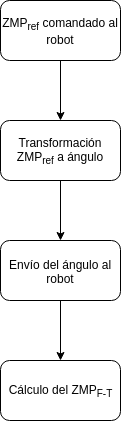
\includegraphics[scale=0.5]{imagenes/apartado_5/52_diagrama_flujo1}
\caption{Diagrama de flujo del programa}
\label{figura52}
\end{figure}


\subsubsection{Respuesta del sistema LIPM}

Se realizaron las pruebas sometiendo al robot a una serie de variaciones en el ángulo de los tobillos para simular perturbaciones pequeñas (empujes), con la excepción de que no volvía al ZMP inicial, para así poder modelar mejor la diferencia entre el ZMP esperado y el medido, estudiándose también su variación dinámica a lo largo del proceso. 

En el presente proyecto se ha llevado a cabo una batería de 30 experimentos en el plano sagital (x-z), representado en la figura \ref{figura53}. Esta metodología también se podría aplicar para cualquier otro plano espacial ya que se obtuvieron resultados similares en el plano frontal (y-z).

\begin{figure}[H]
\centering
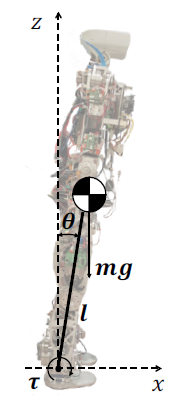
\includegraphics[scale=0.65]{imagenes/apartado_5/53_postura_inicial_experimental_teo}
\caption{Plano de desarrollo de los experimentos del robot TEO}
\label{figura53}
\end{figure}

La arquitectura de control utilizada en los primeros experimentos seguía el siguiente esquema:

\begin{figure}[H]
\centering
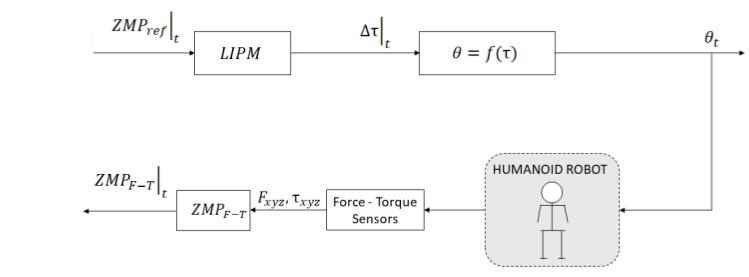
\includegraphics[scale=2.2]{imagenes/apartado_5/54_esquema_bucle_abierto}
\caption{Arquitectura de control de posición básica de ZMP para el modelo LIPM}
\label{figura54}
\end{figure}


En ellos se ajustó la altura del CoM del modelo para reducir lo máximo posible la diferencia entre el ZMP calculado de los F-T y el ZMP deseado. Esta evolución se puede observar de la figura \ref{figura55}, en la que se mejoró la respuesta del sistema pero en la que todavía se mostraba un error en régimen permanente. Como se puede observar, a mayor ZMP el ángulo de inclinación es mayor y el robot es más inestable debido a que éste se encuentra más cerca del borde del polígono de soporte, y los errores tienen mayor influencia, principalmente los que tienen que ver con la flexibilidad de la estructura del robot y sus tolerancias mecánicas. Estos errores se pueden ver en el régimen permanente de la figura \ref{figura55} b). También se observa una oscilación inicial muy grande, algo que se tiene que evitar sobre todo cuando el ZMP se encuentra en el borde del polígono de apoyo. 

\begin{figure}[H]
\centering
\subfigure[altura no ajustada]{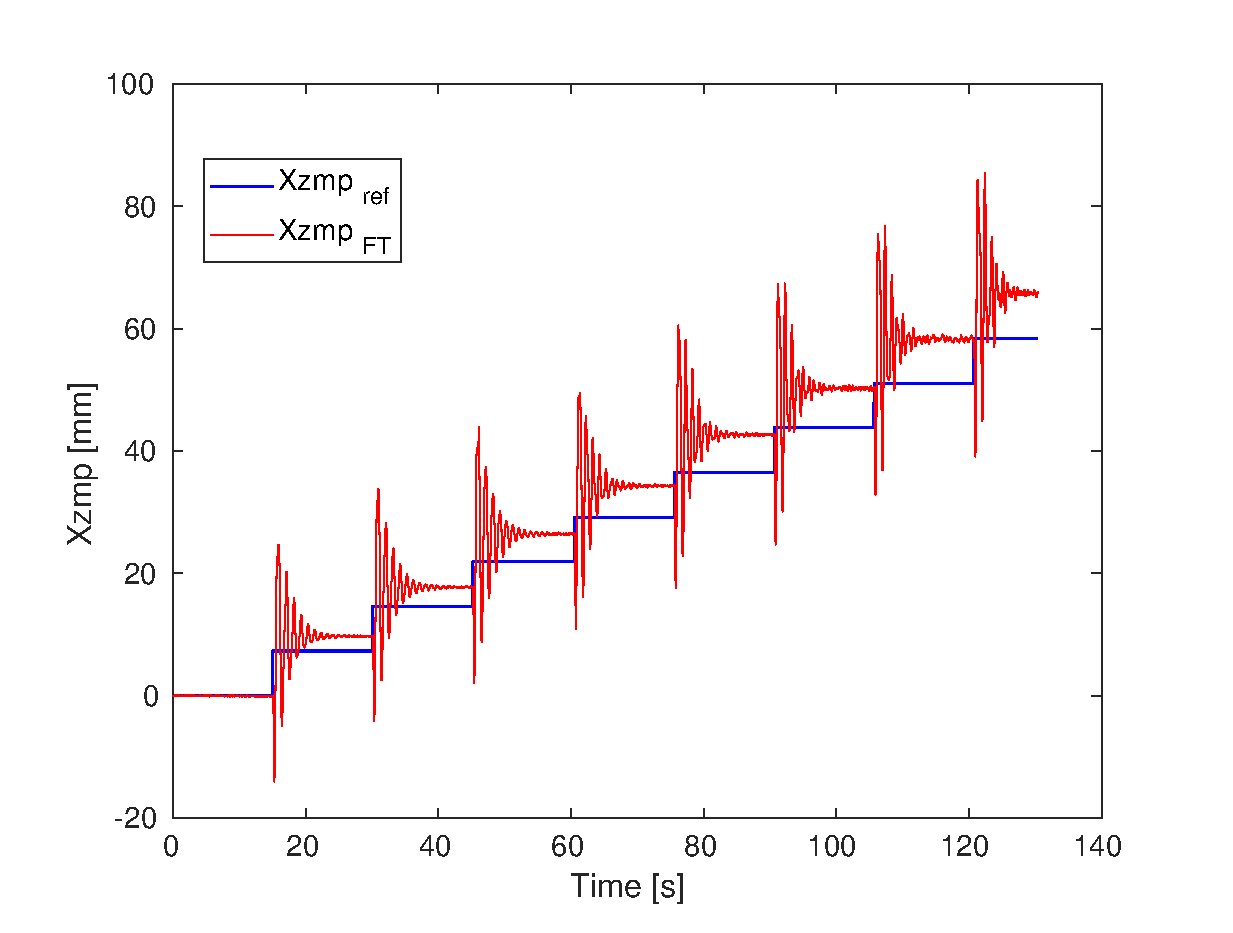
\includegraphics[width=7cm, height=6cm]{imagenes/apartado_5/test6_ft}}
\quad
\subfigure[altura ajustada]{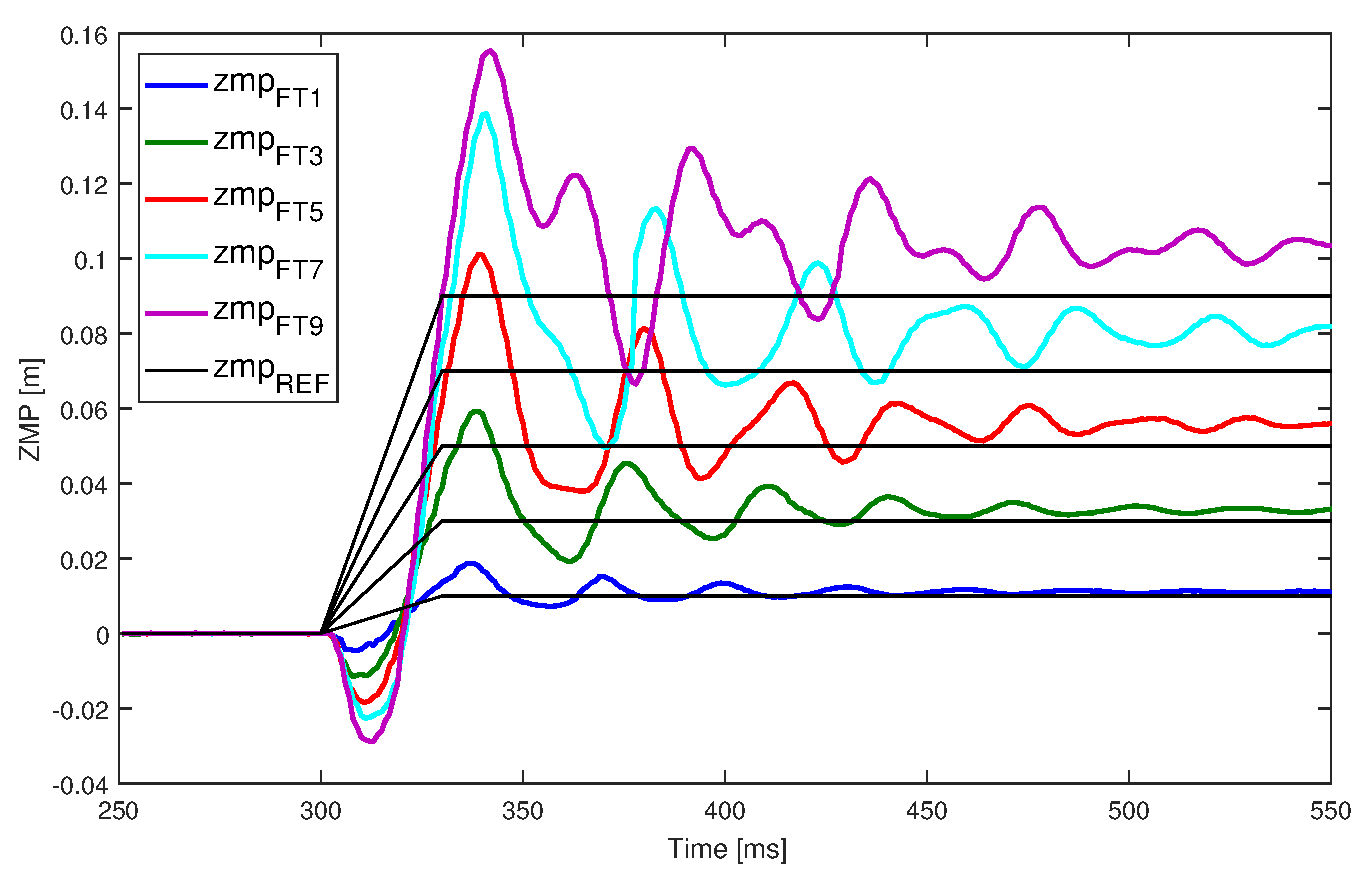
\includegraphics[width=7cm, height=5.9cm]{imagenes/apartado_5/55_2_altura_ajustada.pdf}}
\caption{Evolucion ZMP modelo LIPM}
\label{figura55}
\end{figure}

En los siguientes experimentos, cuya arquitectura de control se muestra en la figura \ref{figura56}, se programó un controlador en ZMP para mejorar la respuesta del sistema y reducir el error tanto en régimen permanente como en el transitorio. Se fueron ajustando diferentes variables de dicho controlador, mostrados en la tabla \ref{tabla51}, para comprobar si el $ZMP_{F-T}$ mejoraba su respuesta tanto en estado estático como en el estado transitorio. 

\begin{figure}[H]
\centering
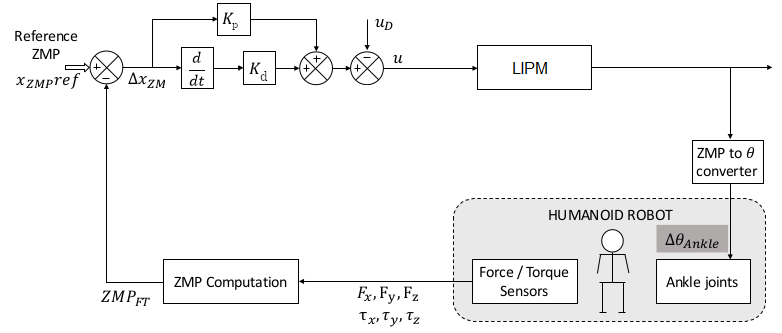
\includegraphics[scale=0.6]{imagenes/apartado_5/56_esquema_bucle_cerrado}
\caption{Arquitectura de control de ZMP mediante controlador PD}
\label{figura56}
\end{figure}


\begin{table}[H]
\begin{center}
\begin{tabular}{|c|c|c|c|}
\hline
Exp. & $k_p$   & $k_d$    & $k_u$ \\ \hline
1    & -0.0025 & 0.00005  & 1    \\ \hline
2    & -0.0025 & 0.00005  & 1.2  \\ \hline
3    & -0.0025 & 0.00005  & 1.4  \\ \hline
4    & -0.0025 & 0.00005  & 2    \\ \hline
5    & -0.005  & 0.0005   & 1    \\ \hline
6    & -0.005  & 0.0005   & 1.65 \\ \hline
7    & -0.01   & 0.0005   & 1    \\ \hline
8    & -0.01   & 0.0005   & 1.65 \\ \hline
9    & -0.05   & 0.005    & 1.65 \\ \hline
10   & -0.015  & -0.00025 & 1.4  \\ \hline
11   & -0.035  & -0.0001  & 1.4  \\ \hline
\end{tabular}
\end{center}
\caption{Batería de experimentos}
\label{tabla51}
\end{table}

\begin{figure}[H]
\centering
\subfigure[Experimento 1]
{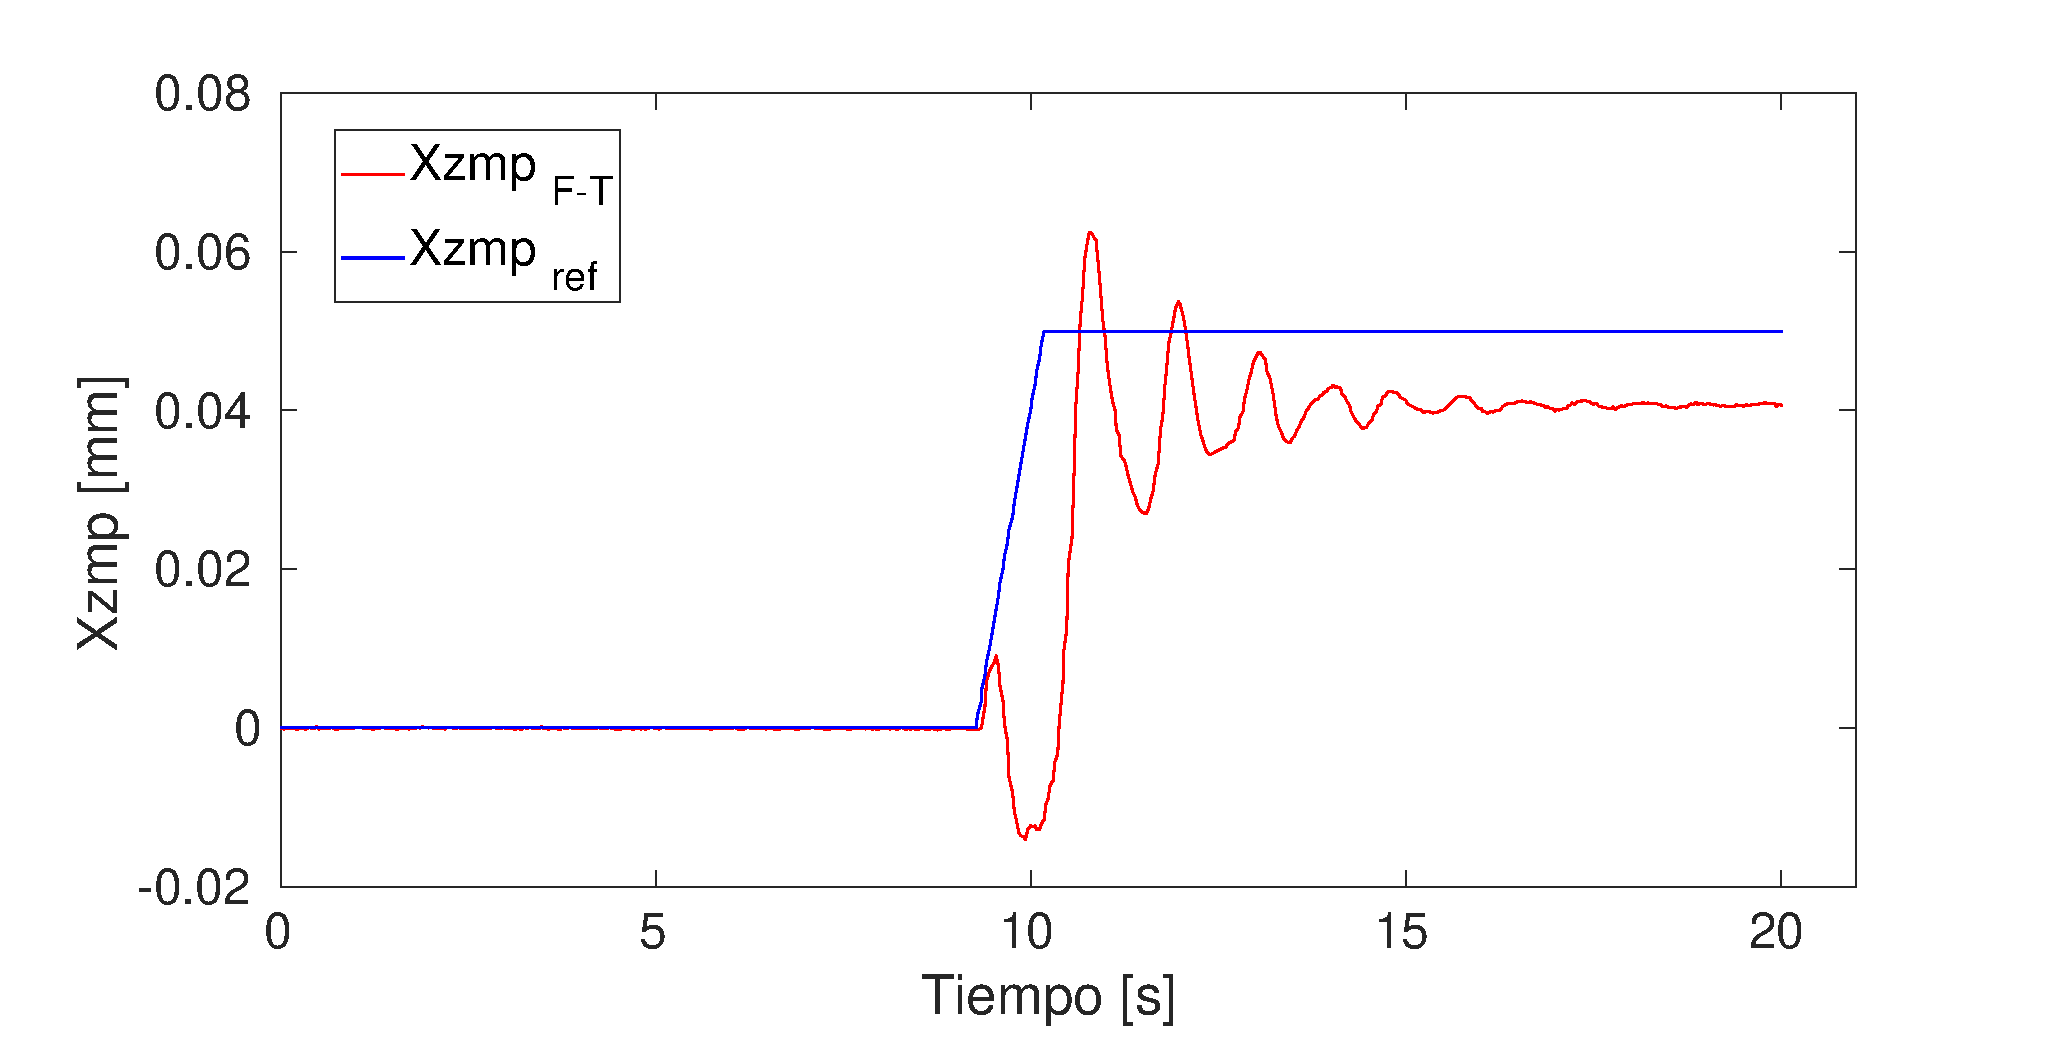
\includegraphics[scale=0.2]{imagenes/apartado_5/57_1_exp1}}
\quad
\subfigure[Experimento 3]
{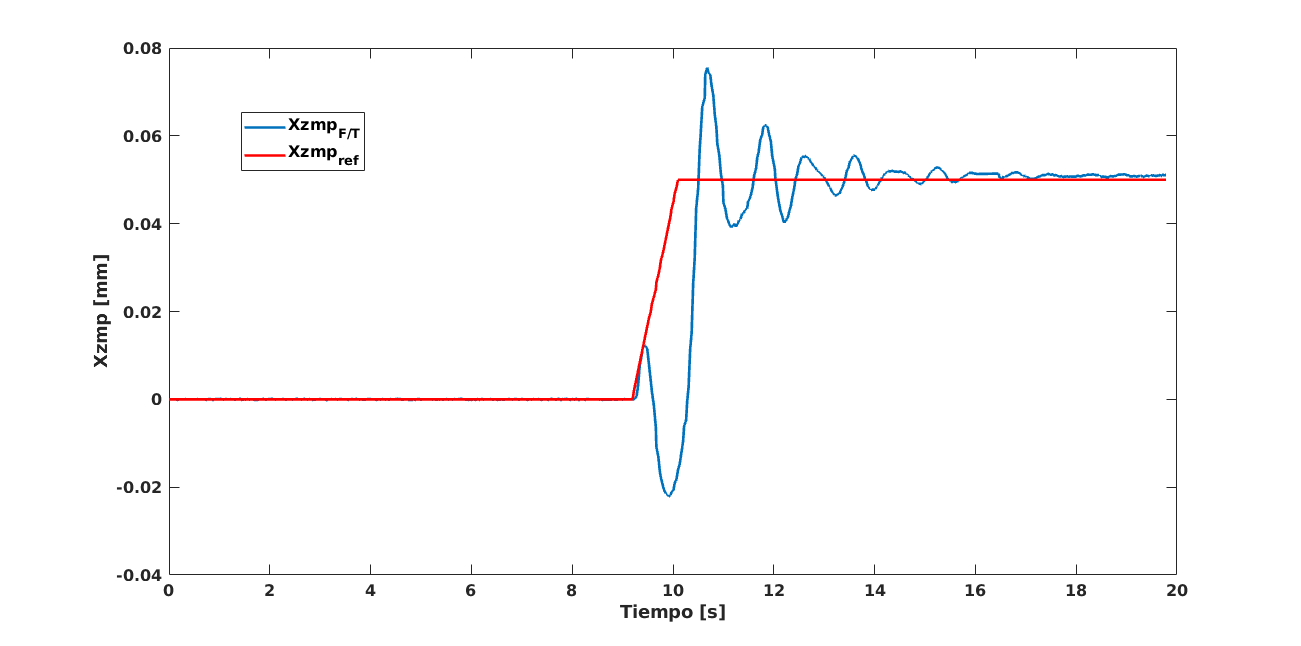
\includegraphics[scale=0.2]{imagenes/apartado_5/57_2_exp3}}
\quad
\subfigure[Experimento 5]
{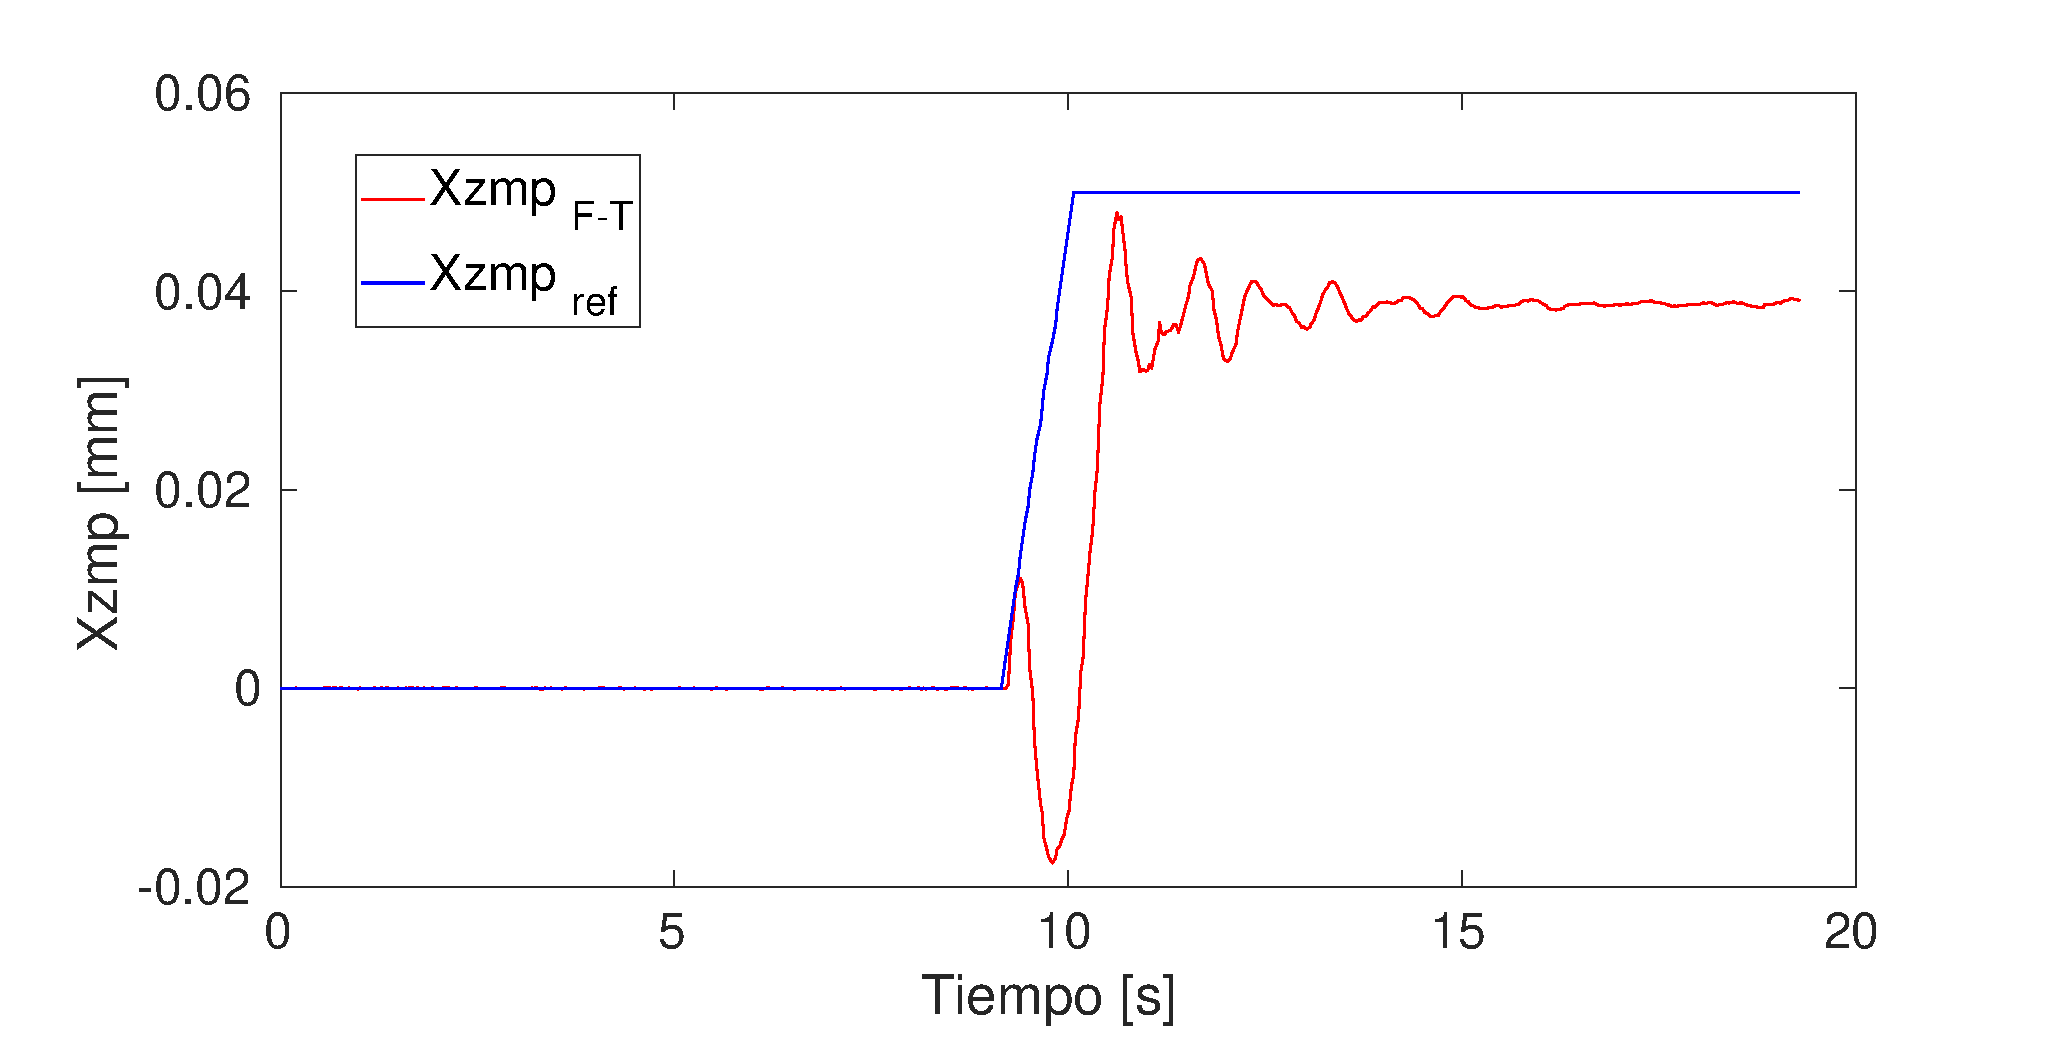
\includegraphics[scale=0.2]{imagenes/apartado_5/57_3_exp5}}
\quad
\subfigure[Experimento 10]
{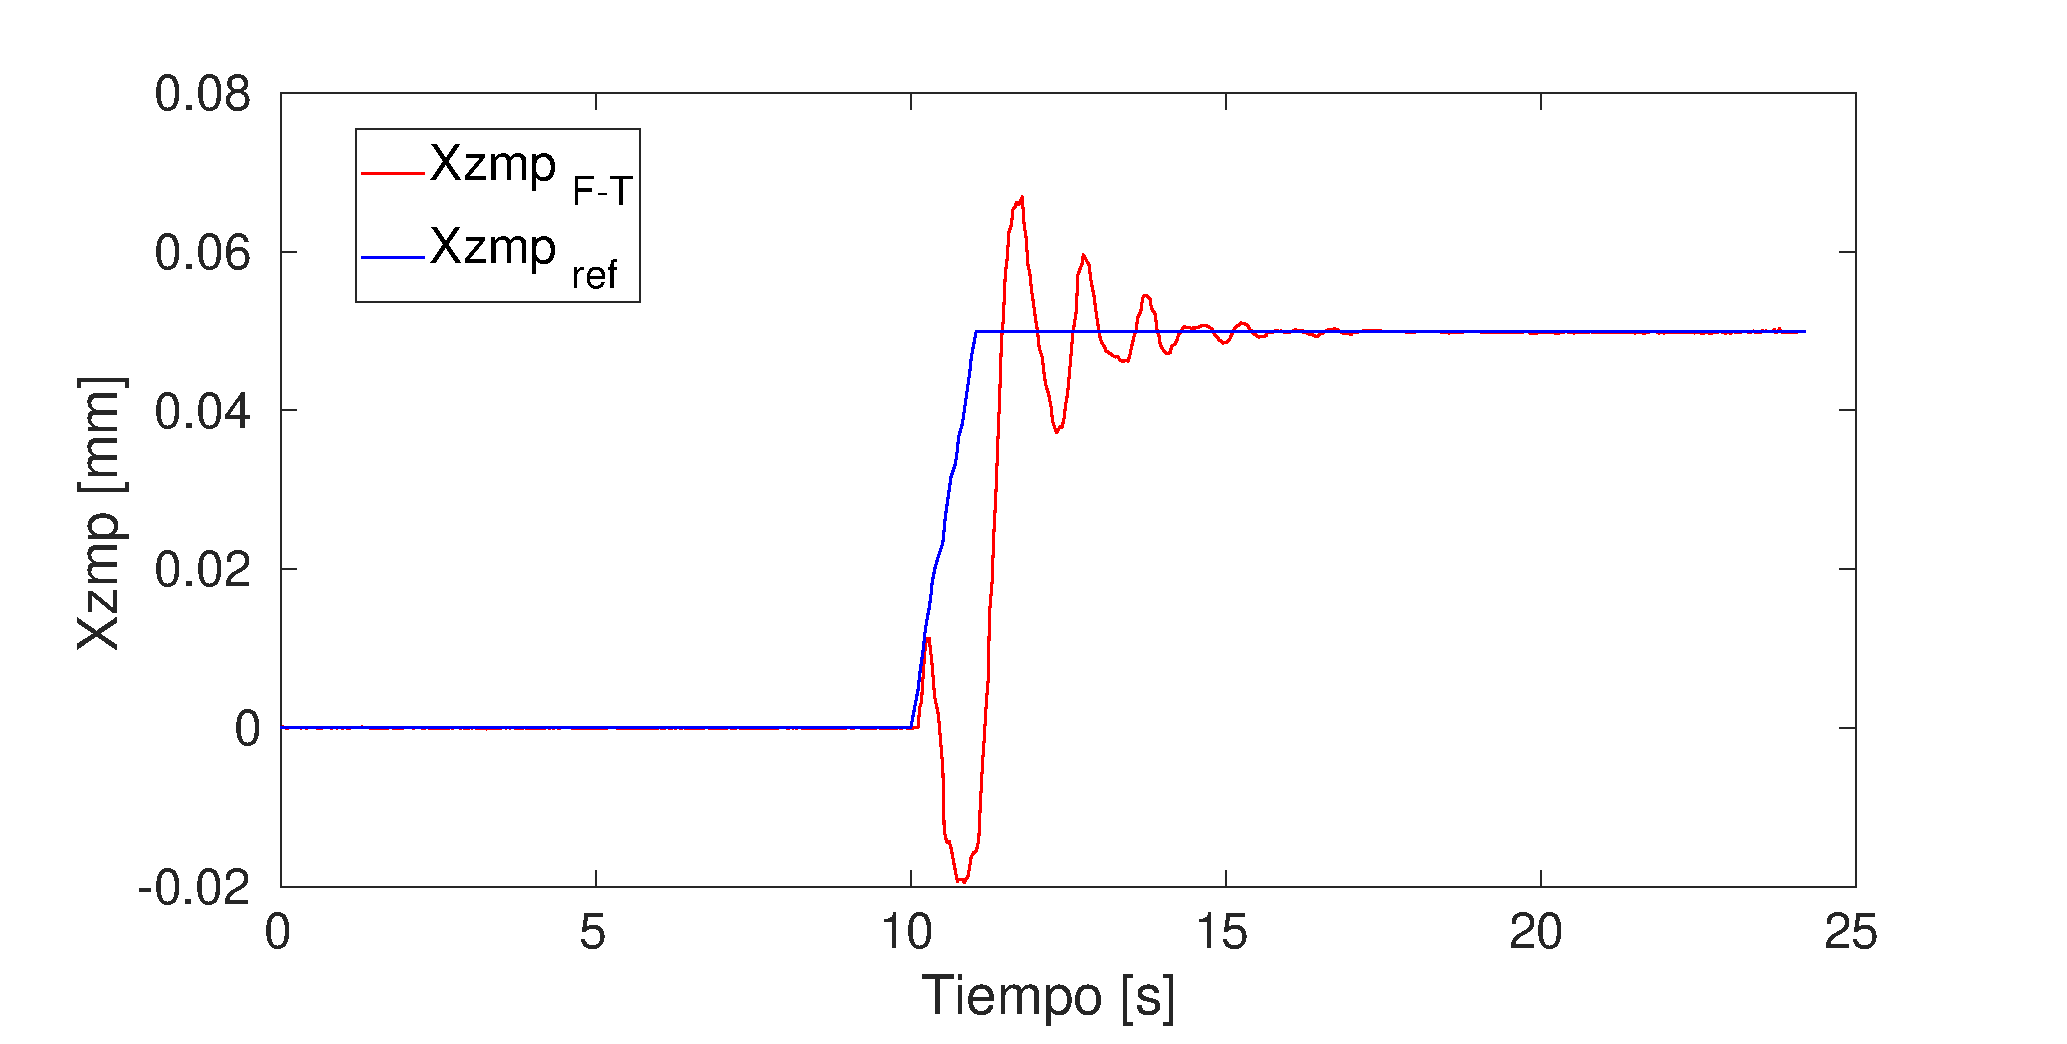
\includegraphics[scale=0.2]{imagenes/apartado_5/57_4_exp10}}
\quad
\subfigure[Experimento 11]
{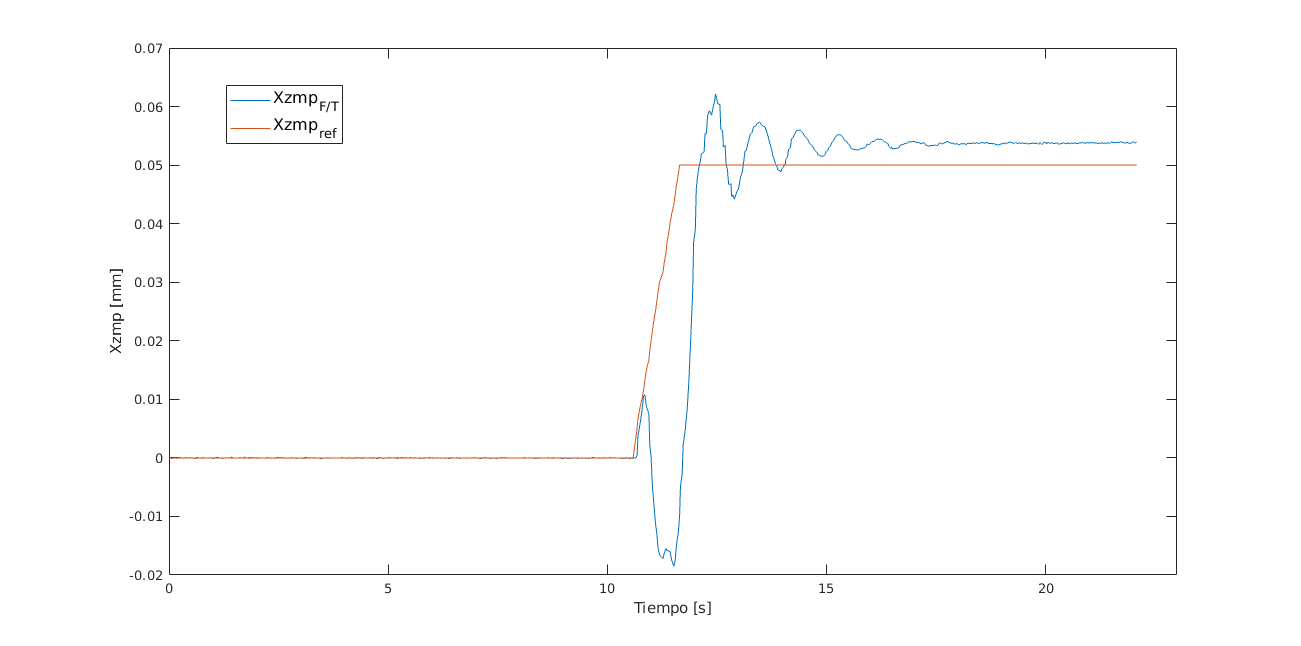
\includegraphics[scale=0.2]{imagenes/apartado_5/57_5_exp11}}
\caption{Evolución ZMP para ZMPref = 5mm}
\label{figura57}
\end{figure}
 

En las pruebas representadas en la figura \ref{figura57}, cuando se lograba ajustar la respuesta en régimen permanente, reduciendo el error entre el $ZMP_{F-T}$ y el ZMP deseado, el régimen transitorio tenía una oscilación muy grande, y como se ha comentado antes esto se tiene que evitar sobre todo en ZMP situados en el borde del polígono de soporte. Por el contrario si se lograba hacer la oscilación inicial un poco más pequeña el tiempo de estabilización del sistema era mayor, por lo que éste se volvía más lento y no se lograba reducir el error del régimen permanente. Es por ello que se hace necesario la mejora del modelo LIPM, tanto para eliminar el error de régimen permanente como para reducir la oscilación y el sobrepaso del régimen transitorio.

\subsubsection{Respuesta del modelo mejorado DLIPM}

Como se ha explicado en el apartado \ref{definicionDLIPM}, se ha aplicado una mejora al modelo LIPM que permitía ajustar de manera dinámica la respuesta del sistema.

Aplicando Laplace a la ecuación de la física del movimiento del nuevo modelo, la función de transferencia quedaría:

\begin{equation*}
-ml{\theta}(S)S^{2} - B_a l{\theta}(S)S - k_a l\theta(S) + mg\theta(S)=- X(S) \cdot mg
\end{equation*}

\begin{equation*}
{\theta}(S)[-ml^{2}S^{2} - B_a lS + (-k_a l + mg)]=- X(S) \cdot mg
\end{equation*}

\begin{equation*}
\frac{{\theta}(S)}{X(S)}=\frac{-mg}{-ml^{2}S^{2} - S B_a l + (-k_a l + mg)}
\end{equation*}

\begin{equation}
\frac{{\theta}(S)}{X(S)}=\frac{\frac{g}{l^{2}}}{S^{2} - S (\frac{B_a}{ml}) + (\frac{k_a}{ml} - \frac{g}{l})}
\label{ec51}
\end{equation}

donde $\gamma=g/l^{2}$, $\alpha=B_{a}/ml$ y $\beta=(k_{a}/ml) - (g/l)$, quedando simplificada:

\begin{equation}
\frac{\theta(S)}{X(S)}=\frac{\gamma}{S^{2}+\alpha S+\beta }
\label{ec52}
\end{equation}

\begin{itemize}

\item \textbf{Caracterización del error en régimen permanente}

El error anteriormente comentado entre el valor deseado de ZMP y el medido, que se detecta en la figura \ref{figura55}b), debe ser caracterizado. Es por ello que en la figura \ref{figura58} se representa dicha desviación a partir de los datos de la figura \ref{figura551} y se realiza su estudio en cada punto experimental ($ZMP_{F-T}$). A partir de dicho estudio se saca una ecuación polinómica de segundo orden para modelar su desviación con respecto al $ZMP_{ref}$:

\begin{equation}
X_{ZMP_{F-T}} = a \cdot X_{ZMP_{ref}} + b \cdot X_{ZMP_{ref}} + c
\label{ec53}
\end{equation}

donde $a=0.834$, $b=1.024$ y $c=-0.0004$.

\begin{figure}[H]
\centering
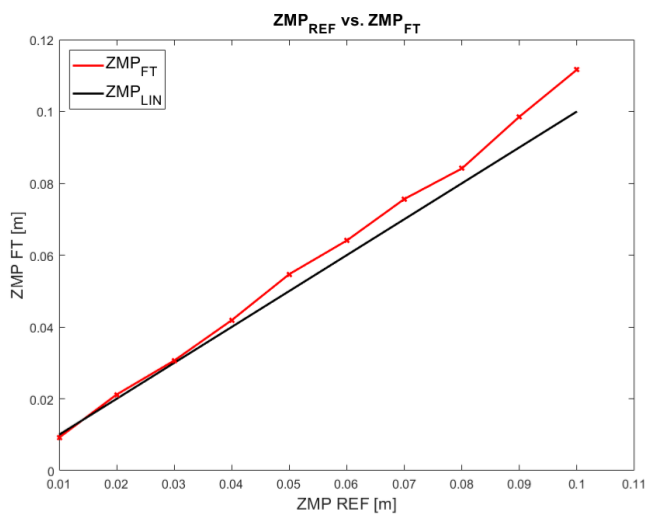
\includegraphics[width=13cm, height=8cm]{imagenes/apartado_5/58_evol_zmp_ft_vs_ref}
\caption{Comparación experimental régimen permanente $ZMP_{F-T}$ y $ZMP_{ref}$}
\label{figura58}
\end{figure}

También sabemos que en régimen permanente, cuando el tiempo tiende a infinito, la ganancia DC del sistema de la ecuación \ref{ec52} queda:

\begin{equation}
\frac{\theta(S)}{X_{ZMP_{F-T}}(S)}|_{S=\infty}=\frac{\frac{g}{l^2}}{\frac{k_a}{ml} - \frac{g}{l}}\Rightarrow K_{DC}=\frac{\gamma}{\beta}
\label{ec54}
\end{equation}

\begin{equation}
X_{ZMP_{F-T}}=\theta_{ref}(\frac{-g^{2}m+k_{a}g}{m})l
\label{ec55}
\end{equation}

Combinando \ref{ec52} y \ref{ec53}, obtenemos $k_a$:

\begin{equation}
k_a=mg(\frac{a \cdot X_{ZMP_{ref}} + b \cdot X_{ZMP_{ref}} + c}{\theta_{ref}\cdot l}+1)
\label{ec56}
\end{equation}

donde,

\begin{equation}
\theta_{ref}=\frac{-180}{\pi}\cdot arcsin(\frac{X_{ZMP_{ref}}}{l})
\label{ec57}
\end{equation}

Una vez que el error estático se ha reducido gracias al parámetro $k_a$, se debe mejorar la respuesta del régimen transitorio para reducir tanto el tiempo de estabilización como el nivel de las oscilaciones iniciales.

\item \textbf{Caracterización de la respuesta transitoria del ZMP}

Se ha demostrado que la respuesta del robot humanoide como péndulo invertido simple es un sistema subamortiguado. En dicho sistema se puede reducir las oscilaciones y modificar su respuesta global seleccionando adecuadamente tanto la ganancia como los parámetros dinámicos. En la figura \ref{figura59}, que muestra la diferencia entre las respuestas de las funciones de transferencia de los modelos LIPM y DLIPM ante una perturbación, se puede visualizar cómo dichos parámetros dinámicos pueden coger valores más altos en el modelo DLIPM, ya que posee un mayor margen de ajuste. 

\begin{figure}[H]
\centering
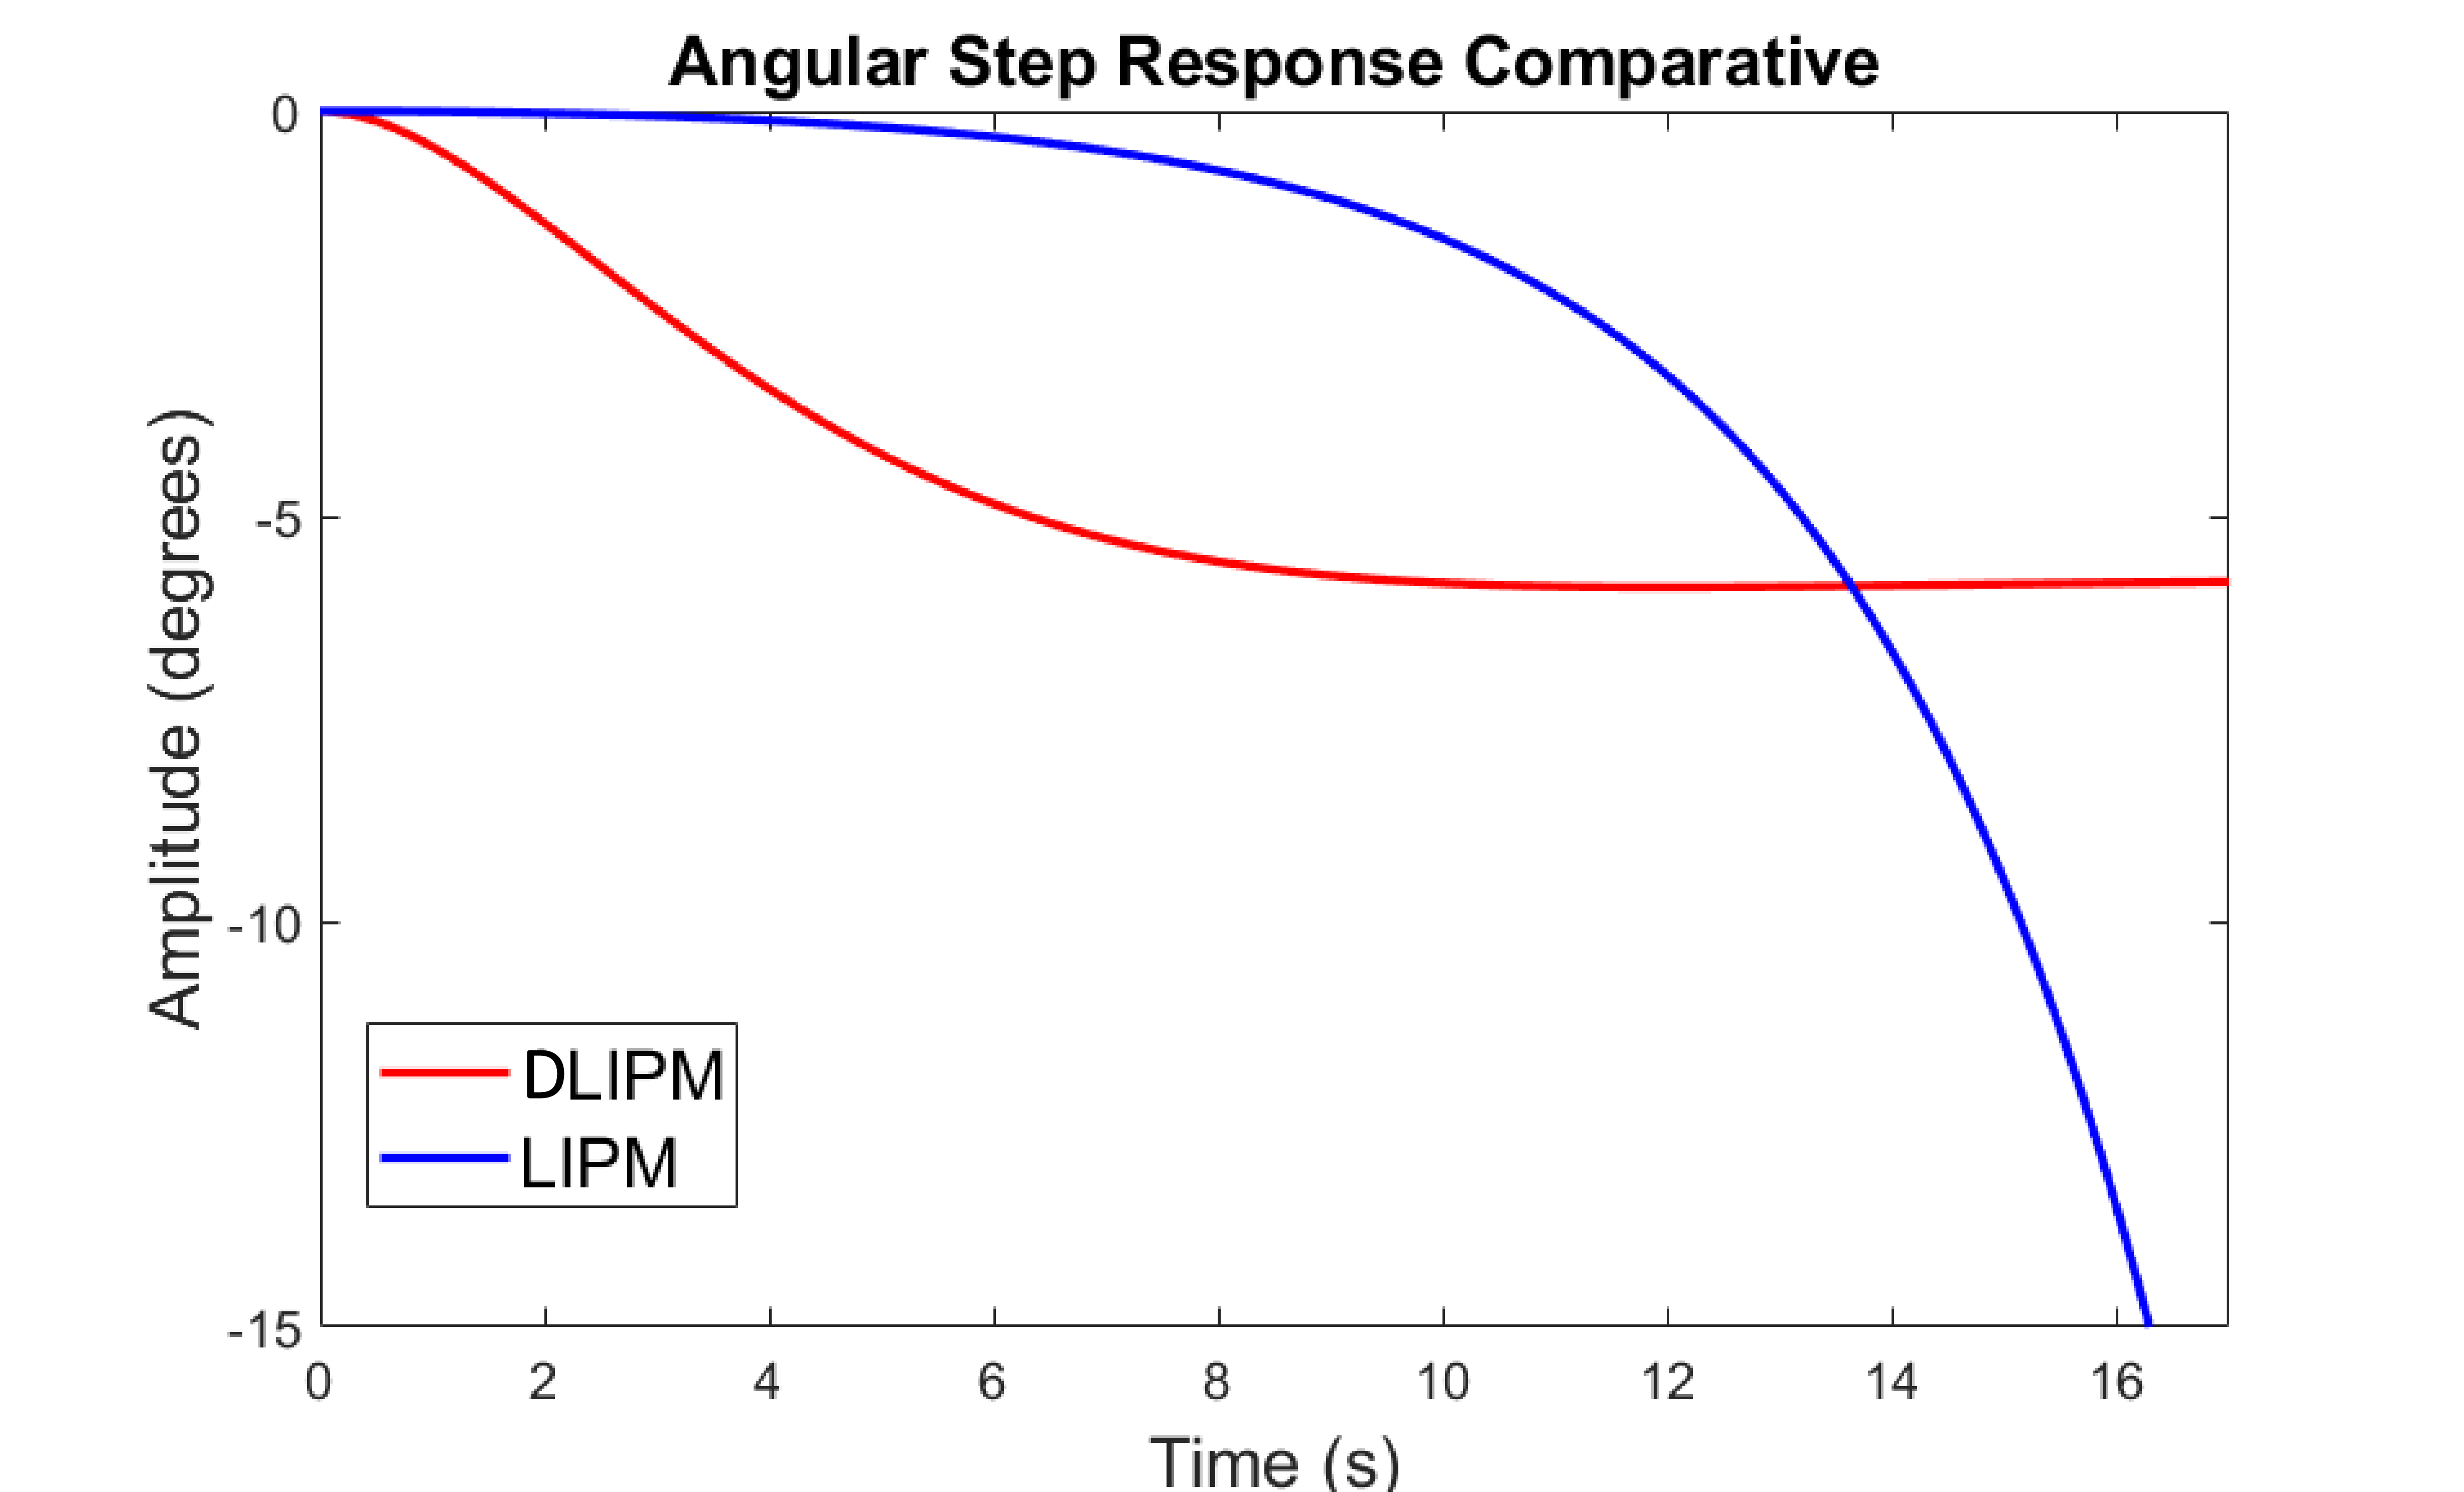
\includegraphics[width=13cm, height=8cm]{imagenes/apartado_5/58_comparativa_paso}
\caption{Comparativa de la respuesta angular entre LIPM y DLIPM}
\label{figura59}
\end{figure}

En el presente proyecto se han escogido unos valores para los parámetros dinámicos de tal manera que han permitido reducir la sobreoscilación. Estos parámetros se obtuvieron de la ecuación \ref{ec52}, ya que $\gamma$ está relacionada con $B_a$, que es el parámetro del modelo DLIPM mediante el cual se puede mejorar la respuesta del sistema en régimen transitorio.

Para un sistema de segundo orden, como es el caso del modelo DLIPM, la función de transferencia en lazo cerrado se escribe como:

\begin{equation}
G(S)=\frac{\theta(S)}{X(S)}=\frac{K{w_{n}}^{2}}{S^{2} + 2\zeta w_{n}S + {w_{n}}^{2}}
\label{ec58}
\end{equation}

donde $w_{n}$ es la frecuencia natural no amortiguada, y $\zeta$, el factor de amortiguamiento relativo del sistema. Para los diferentes valores de $\zeta$, el sistema actuará de diferentes maneras, como se puede observar en la figura \ref{figura59}:

%%imagen sacada de https://electronics.stackexchange.com/questions/135963/why-dont-over-damped-and-critically-damped-circuits-oscillate
\begin{figure}[H]
\centering
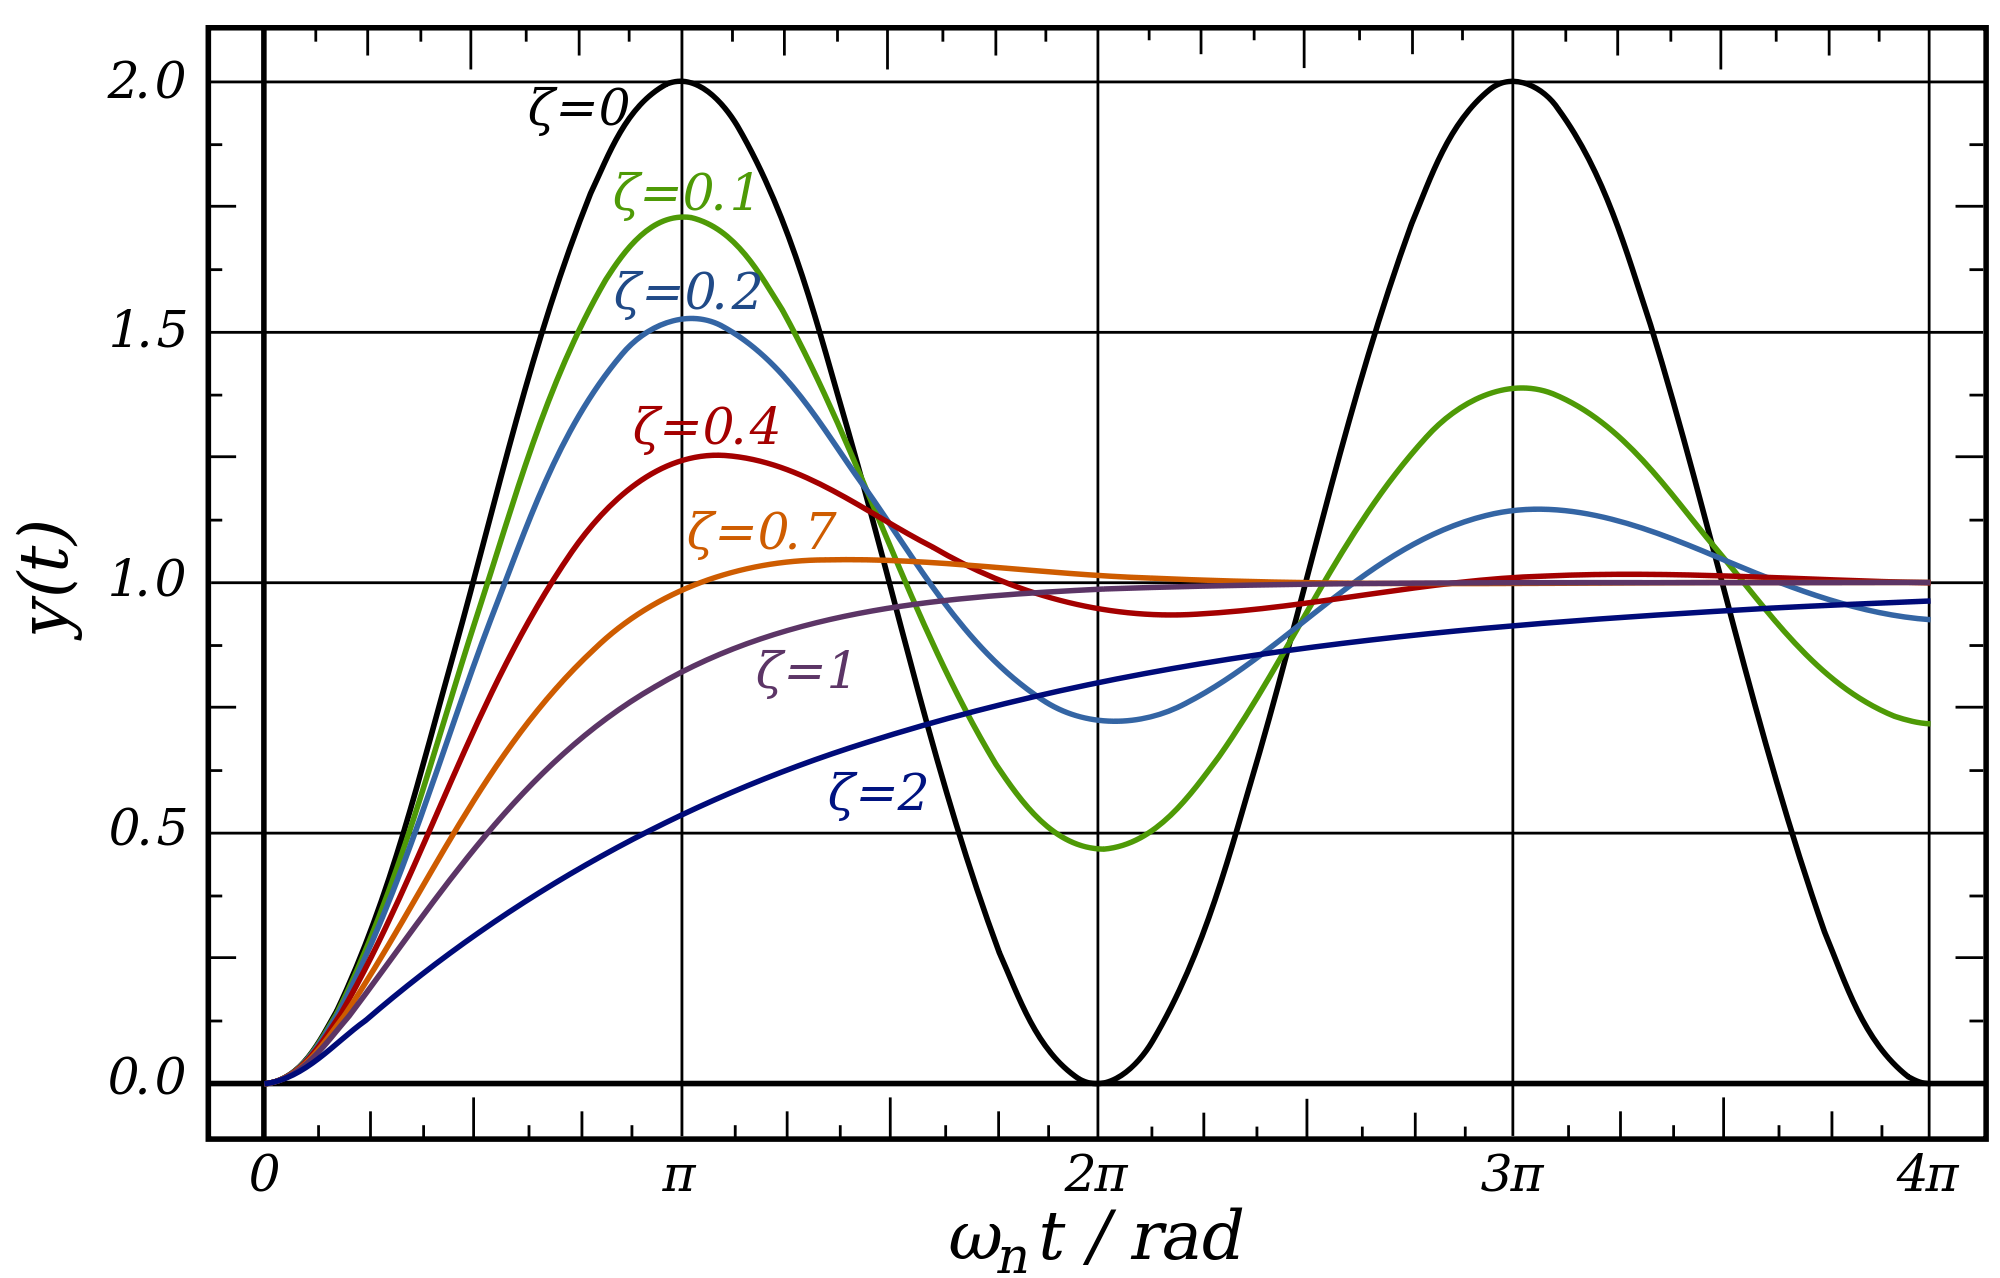
\includegraphics[width=13cm, height=8cm]{imagenes/apartado_5/59_zeta_response_system}
\caption{Respuesta del sistema en función del factor de amortiguamiento}
\label{figura510}
\end{figure}


\begin{enumerate}

\item \textbf{Críticamente amortiguado} $\zeta = 1$

\item \textbf{Sobreamortiguado} $\zeta > 1$

\item \textbf{Subamortiguado} $0 < \zeta < 1$

\end{enumerate}

Igualando \ref{ec51} con \ref{ec58} se obtiene:

\begin{equation}
w_{n}=\sqrt{-\frac{g}{l}+\frac{k_a}{m}}
\label{ec59}
\end{equation}

\begin{equation}
2\zeta w_{n} = \frac{B_a}{m}
\label{ec510}
\end{equation}

En \ref{ec510} como se puede observar hay 2 incógnitas para despejar, por lo que para obtener un resultado debemos fijar una de ellas y despejar la otra. Como se ha comentado antes, el sistema de péndulo invertido es un sistema subamortiguado por lo que se decidió fijar $\zeta$, y despejando de \ref{ec510}, obtenemos $B_a$. Para el actual proyecto, los parámetros dinámicos que se diseñaron fueron $\zeta = 0.8$ y $w_n = 0.4376$.

\begin{figure}[H]
\centering
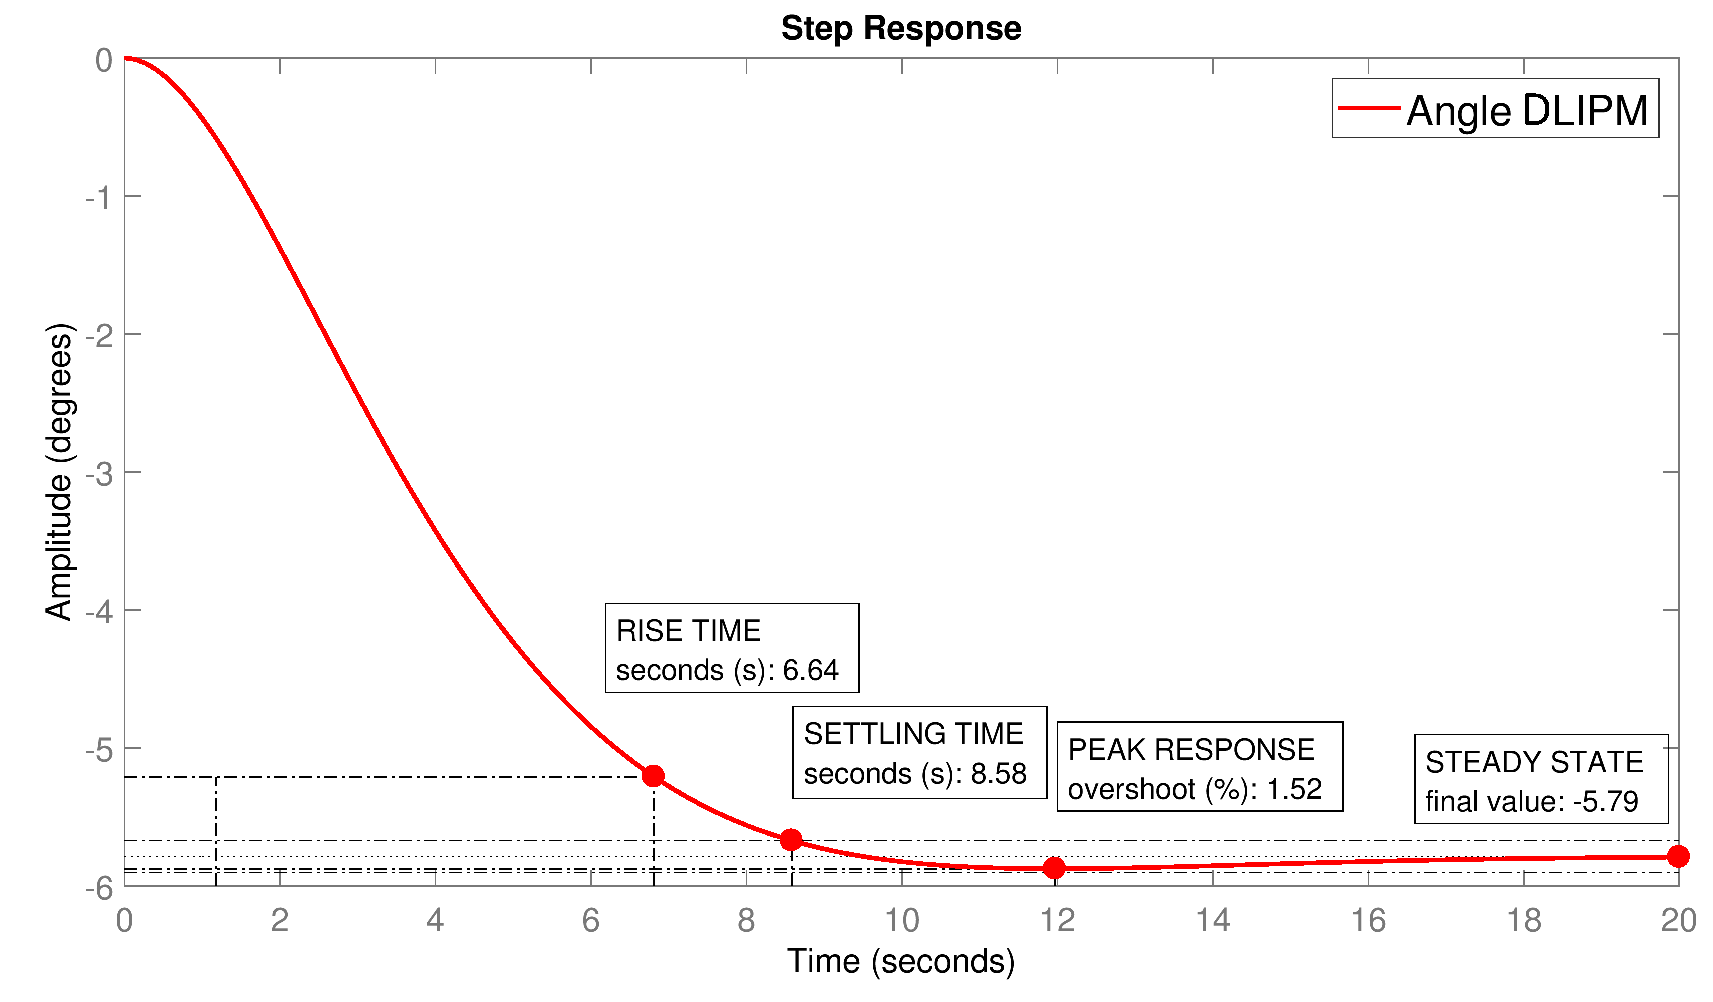
\includegraphics[width=13cm, height=8cm]{imagenes/apartado_5/59_step_response}
\caption{Respuesta angular del modelo DLIPM}
\label{figura511}
\end{figure}

\end{itemize}


\subsubsection{Control de ZMP}

Como el objetivo de este trabajo es abarcar varios puntos de trabajo, se ha propuesto un modelo de controlador no lineal, basado en una ganancia programada, que mediante la selección adecuada de los parámetros dinámicos, permite manejar múltiples puntos de trabajo. Un controlador por ganancia programable es un sistema en el que los parámetros de dicho controlador pueden variar en función de las condiciones de operación o los parámetros de la planta \cite{ref22}. Este controlador utiliza tablas para especificar los valores de la ganancia en función de los parámetros programados.

Las siguientes pruebas se han llevado a cabo siguiendo el esquema de la figura \ref{figura512}, similar a la arquitectura de control utilizada en \cite{ref21}. Para el actual proyecto, dependiendo de la entrada, se pueden seleccionar los valores $k_a$ y $B_a$ adecuados gracias al módulo que permite seleccionar estos parámetros según su planificación. Una vez seleccionados, se calculan los coeficientes de la planta del modelo DLIPM, modificando así su dinámica. Por último, una vez que se ha calculado la planta del modelo DLIPM, éste comanda un ángulo a los tobillos del robot, siendo más progresiva su implementación que en el modelo LIPM.

\begin{figure}[H]
\centering
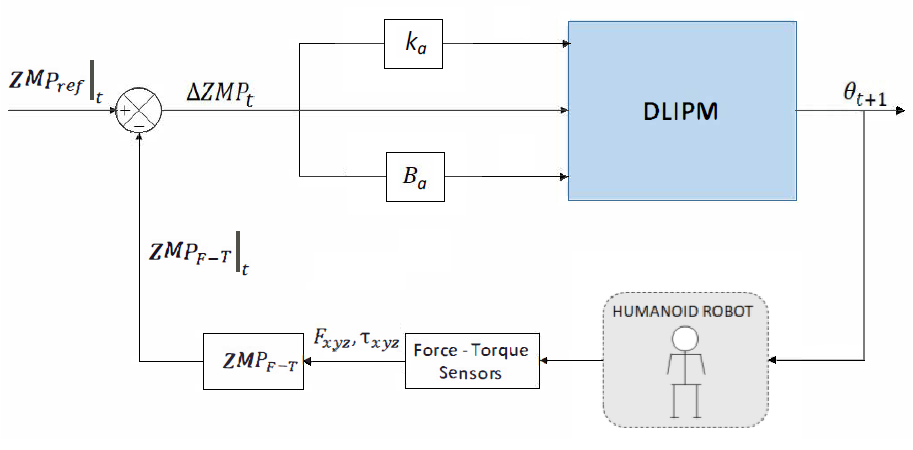
\includegraphics[scale=0.55]{imagenes/apartado_5/510_esquema_DLIPM}
\caption{Arquitectura de control del modelo DLIPM}
\label{figura512}
\end{figure}

\subsubsection{Validación de datos experimentales}

Se realizaron diversos experimentos con el nuevo modelo DLIPM, que consistían en la variación del ZMP deseado para visualizar la respuesta del nuevo sistema de control. Se siguió la misma metodología que para el modelo LIPM.

Para la respuesta en régimen permanente de los experimentos se ha desarrollado la tabla \ref{tabla52}, en la que se muestra una comparación de la ubicación del ZMP deseado y medido entre el modelo LIPM y el modelo DLIPM. Como se puede observar se ha reducido el error estático en todos los puntos de trabajo. Ésta mejora puede observarse de manera gráfica en la figura \ref{figura513}.

\begin{figure}[H]
\centering
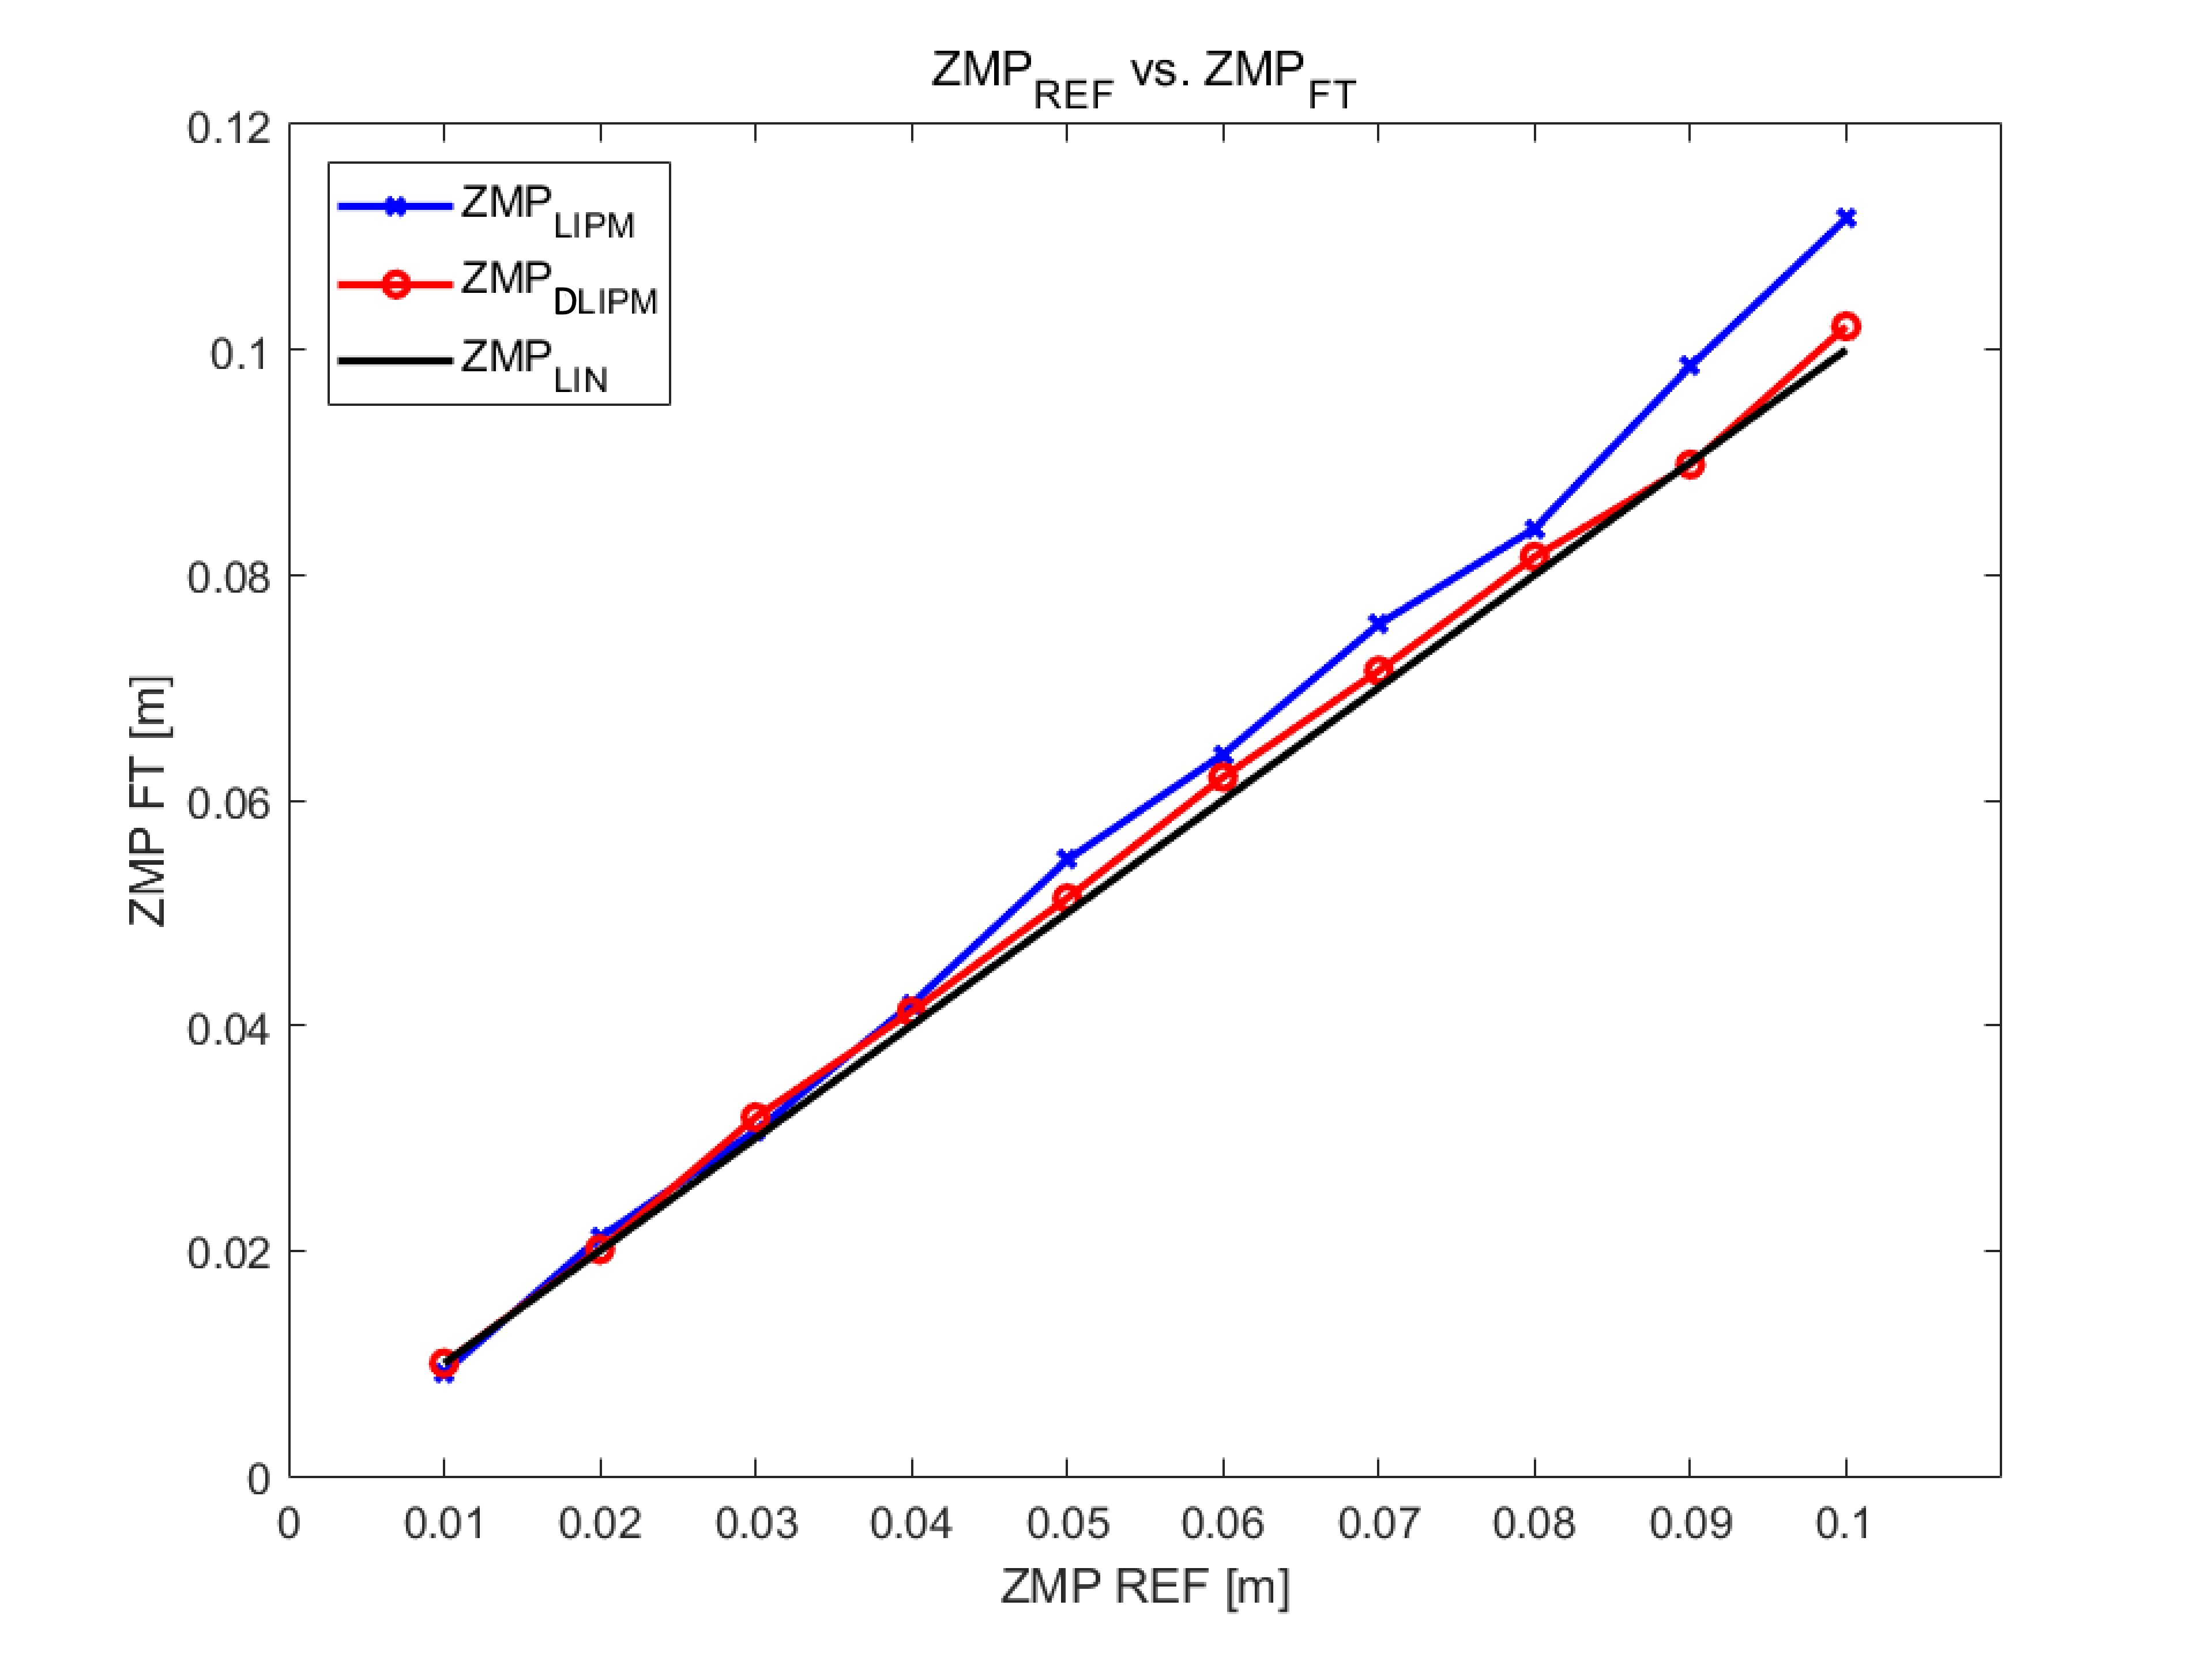
\includegraphics[width=13cm, height=8cm]{imagenes/apartado_5/511_compErrorModels}
\caption{Comparación ZMP de los modelos LIPM y DLIPM}
\label{figura513}
\end{figure}


En cuanto al régimen transitorio, la respuesta se muestra en la figura \ref{figura514}. Se puede observar, comparando ésta con la figura \ref{figura55}, que la respuesta ha mejorado tanto en régimen permanente como en transitorio, reduciendo las oscilaciones, en número pero no tanto en amplitud, y el tiempo de estabilización del robot.

\begin{figure}[H]
\centering
\subfigure[]{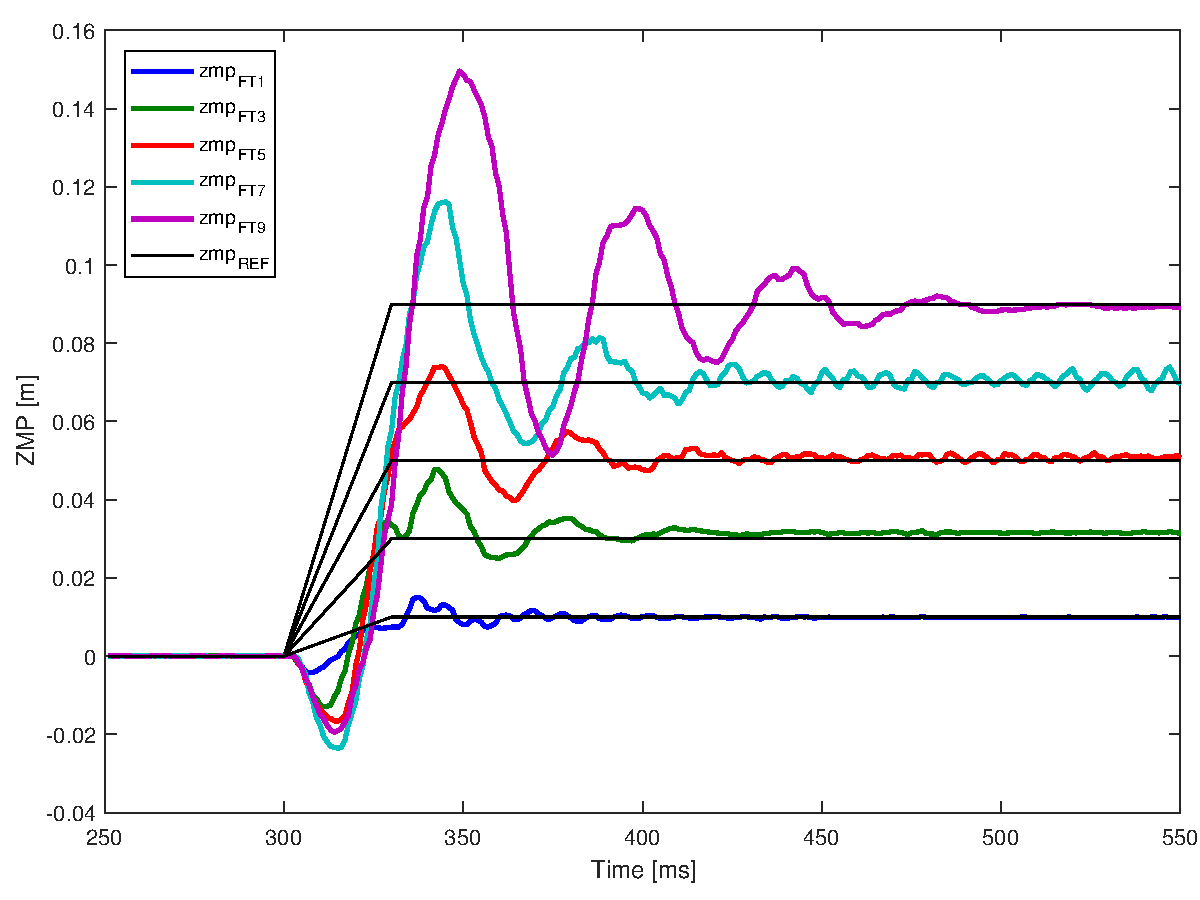
\includegraphics[width=7cm, height=6cm]{imagenes/apartado_5/512_evolucion_zmp_dlipm.pdf}}
\quad
\subfigure[]{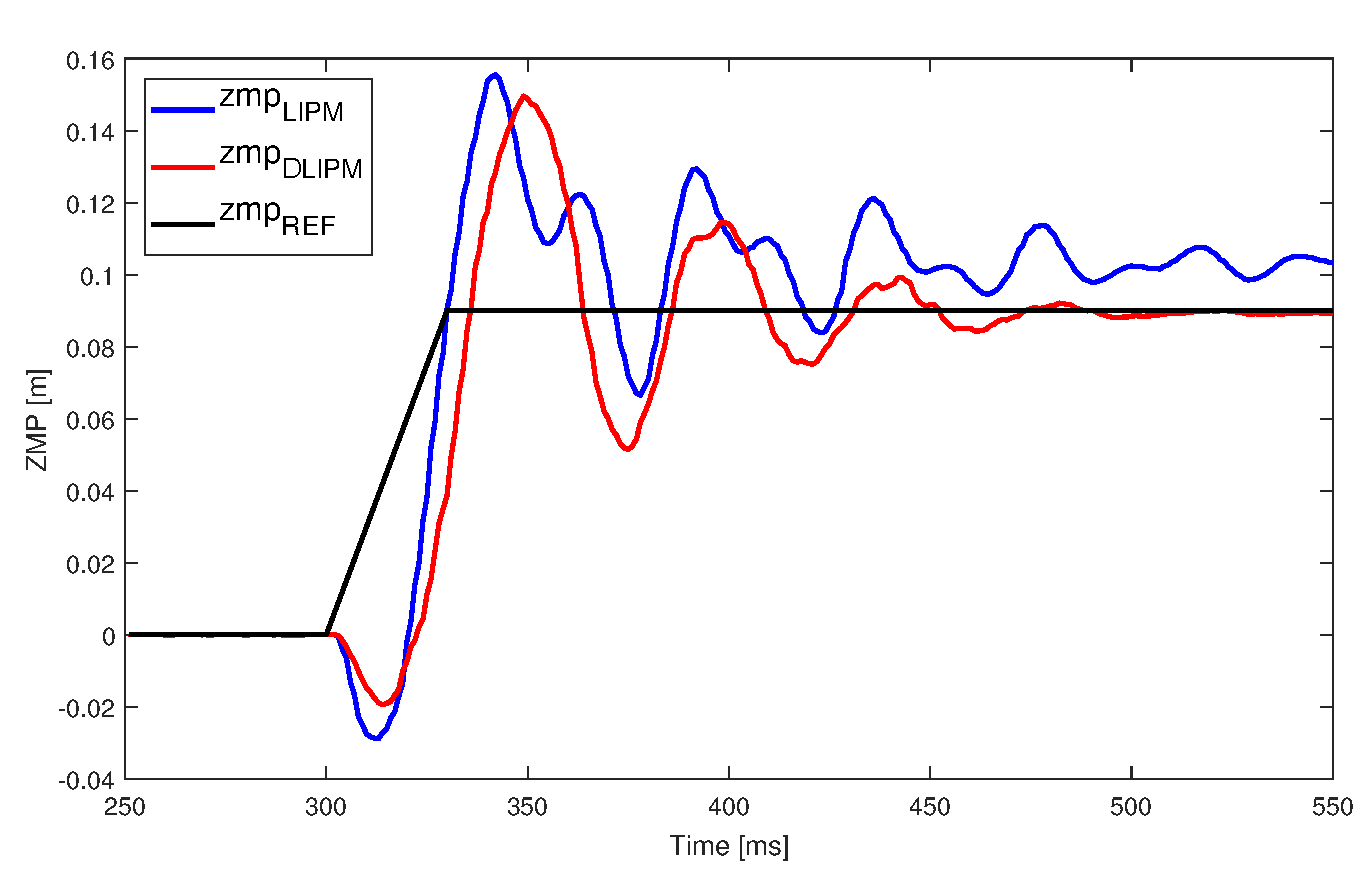
\includegraphics[width=7cm, height=6.2cm]{imagenes/apartado_5/ZMPstep_comparative-eps-converted-to2.pdf}}
\caption{Evolucion ZMP modelo DLIPM. a) Experimentos de la respuesta DLIPM; b) Comparación entre modelo LIPM y DLIPM para $ZMP_{ref} = 9 cm$.}
\label{figura514}
\end{figure}

\subsection{Estudio de la respuesta del sensor inercial IMU}\label{respuestaIMU}

\subsubsection{Descripción de la metodología experimental}

Para los experimentos del modelo cart-table, se siguió la misma metodología de inicio del robot que para el modelo LIPM:

NOTA: Al igual que para las pruebas anteriores, es necesario que en los primeros dos pasos el robot tiene esté en suspensión.

\begin{enumerate}
\item \textbf{Puesta del robot en posición inicial (Homeposs)}

\item \textbf{Corrección offset sensores F-T} 

\item \textbf{Puesta en marcha del sensor inercial IMU}\\ Una vez que se han realizado los dos pasos anteriores, se debe iniciar la IMU para poder obtener datos de aceleraciones del robot para calcular la altura $z_{CoM}$ del modelo cart-table a partir del ZMP del modelo DLIPM. Por último, se baja el robot antes de iniciar el programa.

\item \textbf{Puesta en marcha del programa}\\ Para los experimentos de la IMU se ha desarrollado un programa que iniciase en paralelo el programa del modelo DLIPM y a la vez el del modelo cart-table, tanto para inclinar el robot como para calcular los parámetros necesarios. Como se ha comentado en la sección \ref{equivalencia_modelos}, ambos modelos son equivalentes, por lo que el parámetro de la altura en el modelo cart-table se calculaba a partir del modelo DLIPM, de ahí que los programas se ejecutasen en paralelo, porque se necesitaban los datos de ambos modelos. Una vez que la altura se calculaba, se realizaba el cómputo del ZMP a partir de los datos obtenidos de la IMU. %%Una vez que se ha puesto en marcha el sensor inercial, éste realiza la primera fase igual que en los anteriores experimentos. 
%%\textbf{Corrección offset sensores F-T}\\ Ya realizada la posición de inicio del robot, desde una terminal se deben iniciar los sensores F-T de los tobillos que se van a encargar de dar la información de las fuerzas y los pares al programa para así poder realizar los experimentos, siempre con el robot en suspensión para eliminar los posibles offset que puedan tener los mismos. Es importante que no esté apoyado en el suelo para que cuando se ejecute esta corrección, no se elimine el valor de la fuerza ejercida por la masa del robot. Una vez que se han iniciado los sensores F-T de los tobillos ya se podría bajar el robot para que éstos puedan tener en cuenta el propio peso del robot y las demás fuerzas y pares.
\end{enumerate}

\subsubsection{Respuesta del modelo cart-table}

Como se ha comentado en el apartado \ref{equivalencia_modelos}, tanto el modelo de péndulo invertido simple como el cart-table son distintas formas de computar el ZMP. En \cite{ref22} el modelo cart-table presentaba errores en régimen permanente, como se puede observar en \ref{figura515}.


\begin{figure}[H]
\centering
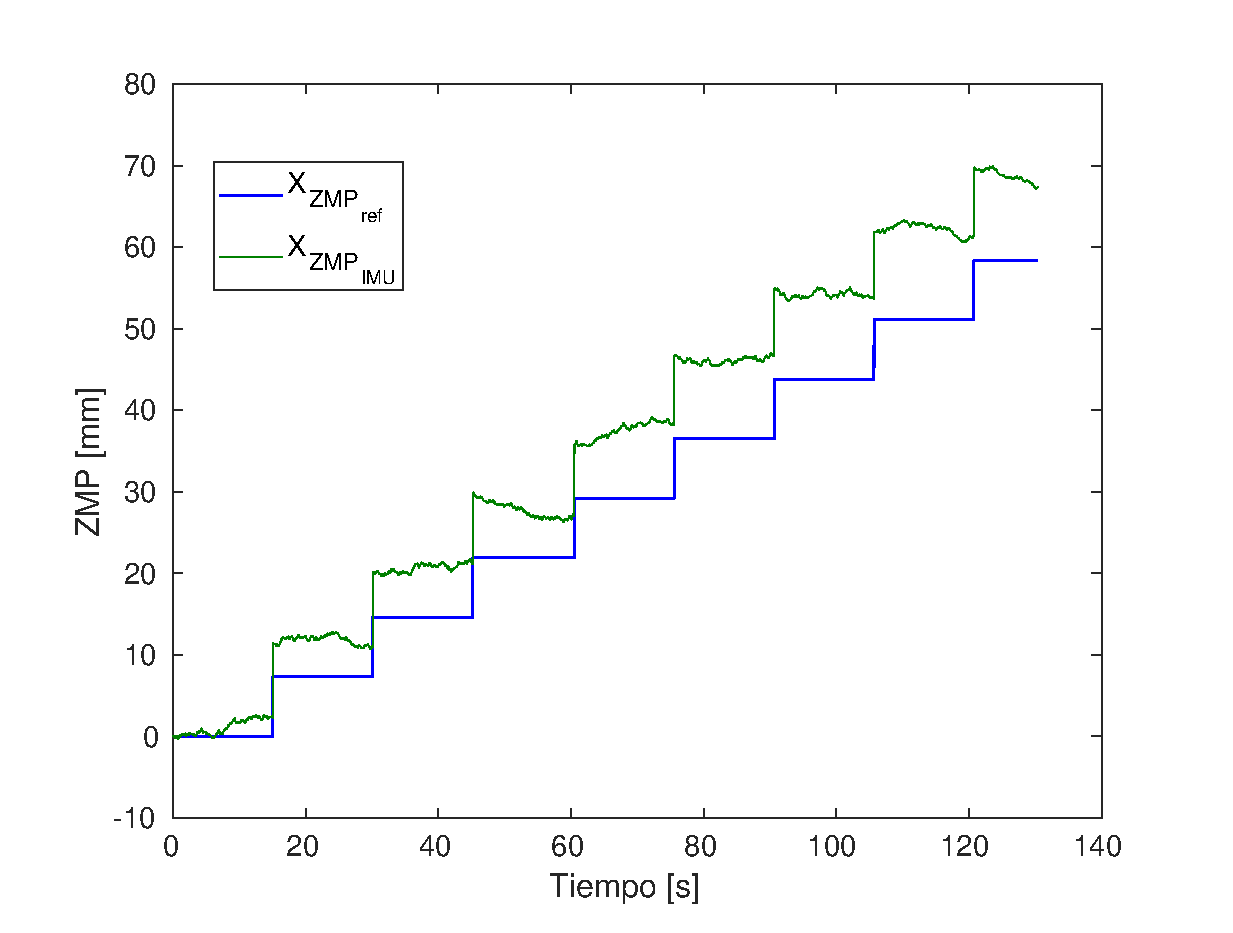
\includegraphics[width=13cm, height=8cm]{imagenes/apartado_5/test6_imu2}
\caption{Evolucion ZMP modelo cart-table}
\label{figura515}
\end{figure}

Se hizo el estudio de ambos modelos para averiguar los parámetros más importantes de ambos modelos. Se observó que la altura del CoM necesitaba ser modificada en el modelo cart-table para que ambos modelos dieran el mismo ZMP.

Una vez que se computó la altura del modelo cart-table, se volvieron a hacer las pruebas, mejorando su respuesta en régimen permanente. La corrección de dicho error en régimen permanente puede observarse en la figura \ref{figura516} en la que se indica de color negro la referencia a la que debían llegar los ZMP tanto del modelo DLIPM (en rojo) como el modelo cart-table (en verde).

\begin{figure}[H]
\centering
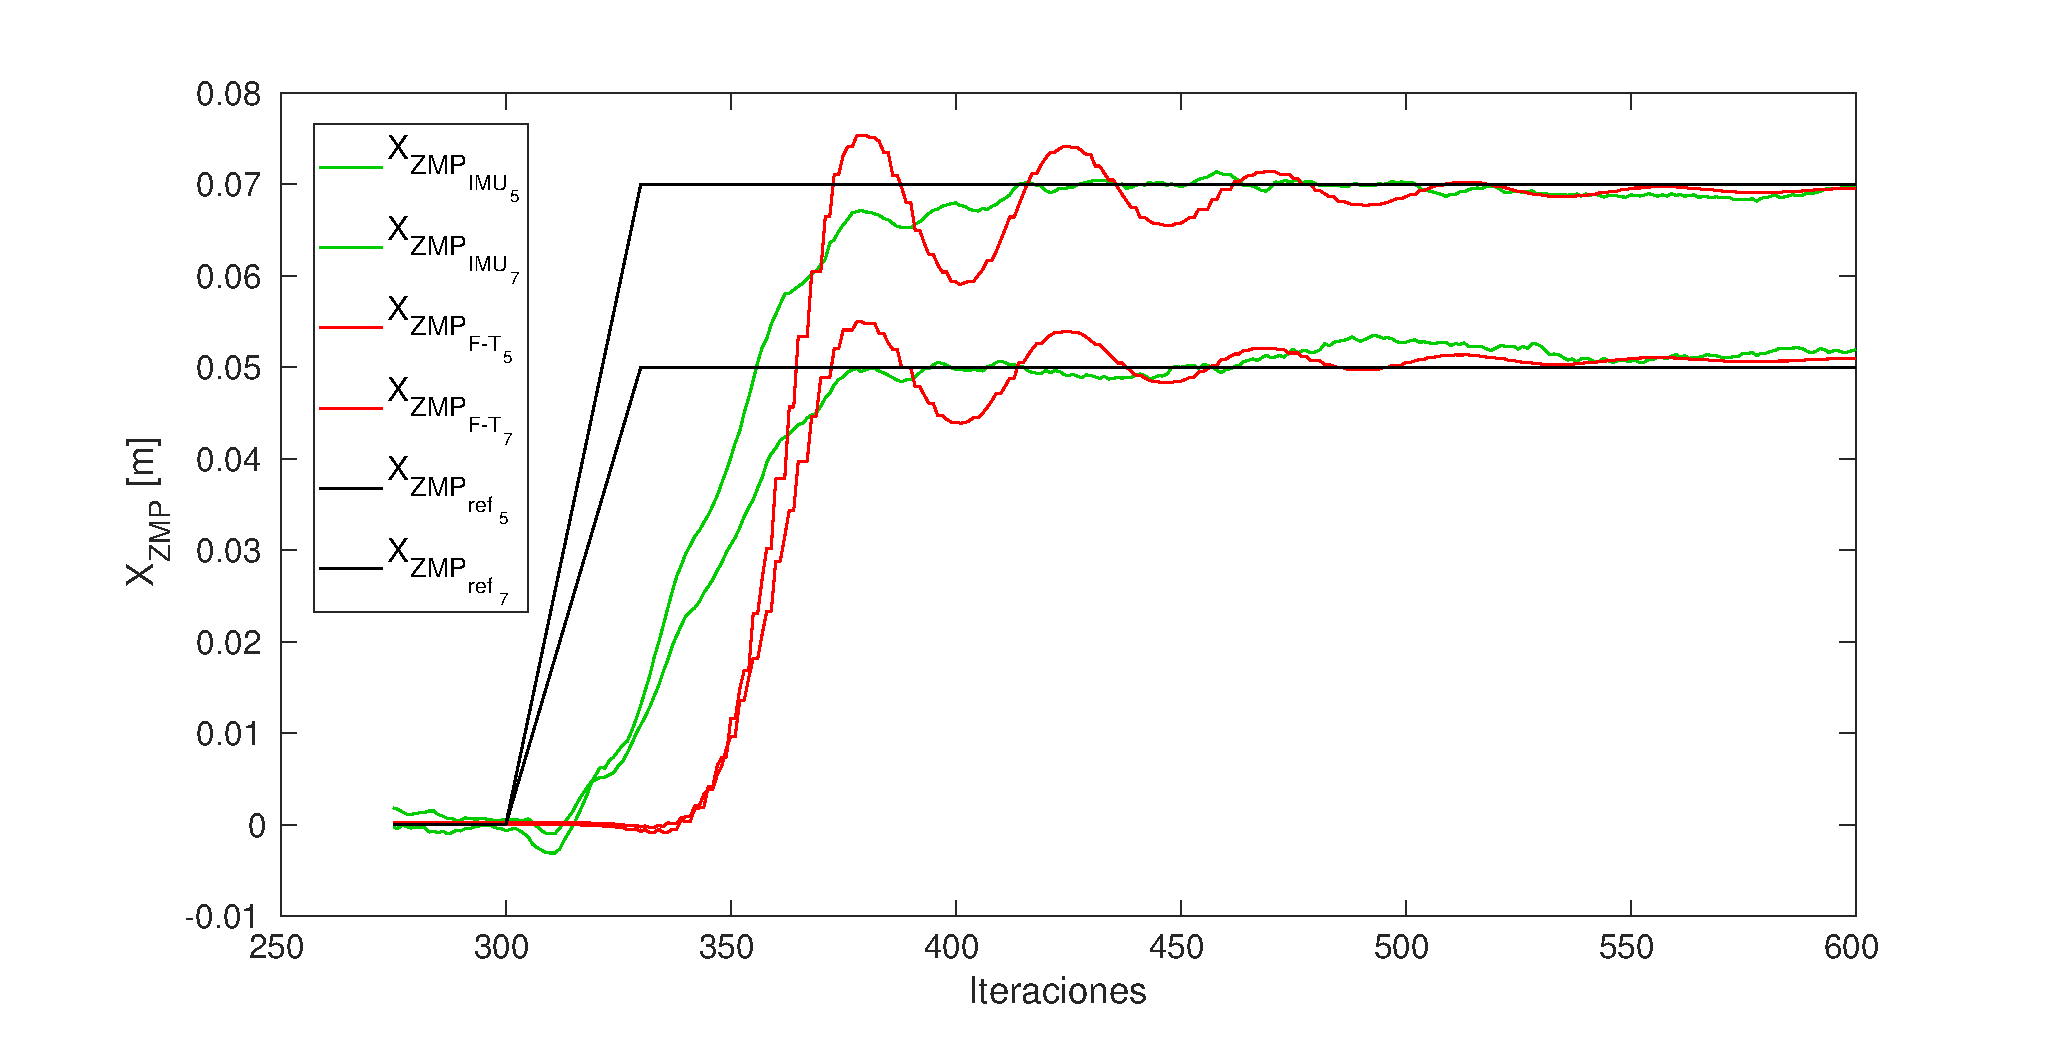
\includegraphics[width=13cm, height=8cm]{imagenes/apartado_5/test2_imu}
\caption{Representación ZMP modelo cart-table corregido}
\label{figura516}
\end{figure}

\begin{figure}[H]
\centering
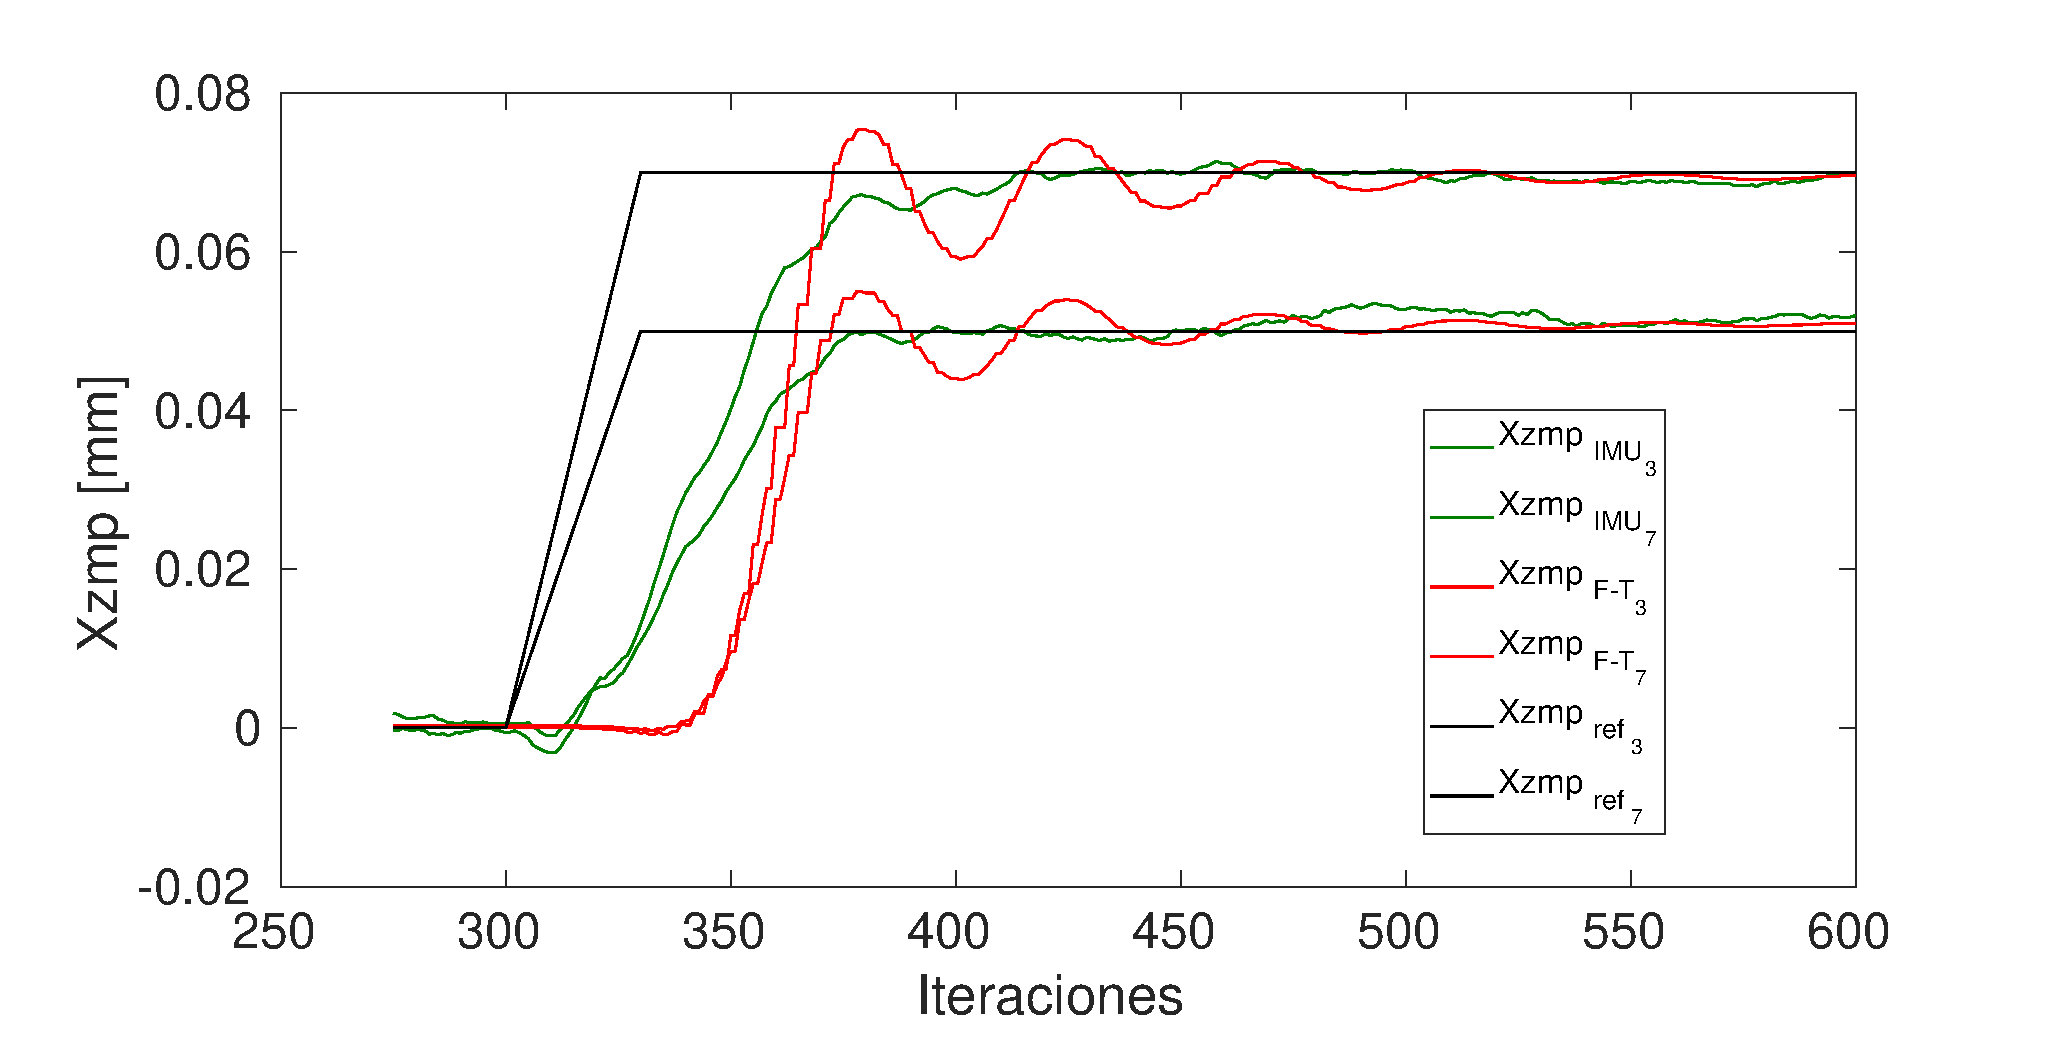
\includegraphics[width=13cm, height=8cm]{imagenes/apartado_5/test_allcsv4_2}
\caption{Representación ZMP modelo cart-table corregido}
\label{figura516}
\end{figure}



\afterpage{\null\newpage}
\newpage
